%%%%%%%%%%%%%%%%%%%%%%%%%%%%%%%%%%%%%%%%%%%%%%%%%%%%%%%%%%%%%%%%%
%%%%%%%%%%%%%%%%%%% Main Thesis TeX Document %%%%%%%%%%%%%%%%%%%%
%%%%%%%%%%%%%%%%%%%%%%%%%%%%%%%%%%%%%%%%%%%%%%%%%%%%%%%%%%%%%%%%%
\documentclass[12pt,oneside]{report}
\usepackage{
    gsuthesisETD,
    multicol,
    amssymb,
    amsthm,
    amsmath,
    graphicx,
    geometry,
    float,
    times,
}
\newcommand{\theoremheaderfont}{\scshape}
\geometry{
    letterpaper,
    left=1.5in,
    right=1in,
    top=1in,
    bottom=1in,
    headheight=12pt,
    headsep=20pt,
    footskip=1in
}


%%%%%%%%%%%%%%%%%%%%%%%%%%%%%%%%%%%%%%%%%%%%%%%%%%%%%%%%%%%%%%%%%
%%%%%%%%%%%%%%%%%%%% %Toggles: "true" or "false" %%%%%%%%%%%%%%%%
%%%%%%%%%%%%%%%%%%%%%%%%%%%%%%%%%%%%%%%%%%%%%%%%%%%%%%%%%%%%%%%%%
\tablespagetrue
\figurespagetrue
%\symbolpagetrue
%\dedicationpagetrue
\acknowledgmentspagetrue
\copyrightpagetrue
\sectionnumberstrue


%%%%%%%%%%%%%%%%%%%%%%%%%%%%%%%%%%%%%%%%%%%%%%%%%%%%%%%%%%%%%%%%%
%%%%%%%%%%%%%%%%%%%%% Fill in These Fields %%%%%%%%%%%%%%%%%%%%%%
%%%%%%%%%%%%%%%%%%%%%%%%%%%%%%%%%%%%%%%%%%%%%%%%%%%%%%%%%%%%%%%%%
\title{Bias of Rank Correlation Under a Mixture Model}
\author{Russell Charles Land}
\degree{Master of Science}
\major{Mathematics}
\dept{Mathematical Sciences}
\school{Georgia Southern University}
\thesistype{Thesis}
\graduatedate{May 2021}
\graduateyear{2021}
\keywords{
    Rank correlation,
    Copula,
    Mixture model,
    Spearman Rho,
    Kendall Tau,
    Cumulative distribution function,
    Bias
}
\msc{15A15, 41A10}
\cochair=0
%\symbolfile{symbols}
\appendname{APPENDIX}
\tocheader{Appendices}
\mybibname{REFERENCES}
\def\deansname{Dr. Stephen Carden}
\committeechair{Stephen Carden}
\memberB{Divine Wanduku}
\memberC{Arpita Chatterjee}
\degreeA{M.S., Georgia Southern University, 2021}
\degreeB{B.S., Georgia Southern University, 2019}


%%%%%%%%%%%%%%%%%%%%%%%%%%%%%%%%%%%%%%%%%%%%%%%%%%%%%%%%%%%%%%%%%
%%%%%%%%%%%%%%%%%%%%%%%%% MACROS %%%%%%%%%%%%%%%%%%%%%%%%%%%%%%%%
%%%%%%%%%%%%%%%%%%%%%%%%%%%%%%%%%%%%%%%%%%%%%%%%%%%%%%%%%%%%%%%%%
\newtheorem{theorem}{Theorem}[chapter]
\newtheorem{definition}[theorem]{Definition}
\newtheorem{corollary}[theorem]{Corollary}
\newtheorem{lemma}[theorem]{Lemma}
\newtheorem{remark}[theorem]{Remark}
\newtheorem{prop}[theorem]{Proposition}
\newtheorem{example}[theorem]{Example}
\newtheorem{ass}[theorem]{Assumption}


%%%%%%%%%%%%%%%%%%%%%%%%%%%%%%%%%%%%%%%%%%%%%%%%%%%%%%%%%%%%%%%%%
%%%%%%%%%%%%%%%%%%%%%%%%% MISCELLANEOUS %%%%%%%%%%%%%%%%%%%%%%%%%
%%%%%%%%%%%%%%%%%%%%%%%%%%%%%%%%%%%%%%%%%%%%%%%%%%%%%%%%%%%%%%%%%
\usepackage{mdframed,hyperref}
\setlength\parindent{24pt}
\DeclareMathOperator{\ran}{ran}
\DeclareMathOperator{\dom}{dom}
\DeclareMathOperator{\sign}{sign}
\allowdisplaybreaks
\bibliographystyle{ieeetr}
\hypersetup{
    colorlinks,
    citecolor=black,
    filecolor=black,
    linkcolor=black,
    urlcolor=black
}
\renewcommand{\qedsymbol}{$\blacksquare$}


%%%%%%%%%%%%%%%%%%%%%%%%%%%%%%%%%%%%%%%%%%%%%%%%%%%%%%%%%%%%%%%%%
%%%%%%%%%%%%%%%%%%%%%%%%% Main Document %%%%%%%%%%%%%%%%%%%%%%%%%
%%%%%%%%%%%%%%%%%%%%%%%%%%%%%%%%%%%%%%%%%%%%%%%%%%%%%%%%%%%%%%%%%
\begin{document}

  \begin{abstract}

\noindent This thesis project will analyze the bias in mixture models when contaminated data is present. Specifically, we will analyze the relationship between the bias and the mixing proportion, $p$, for the rank correlation methods Spearman's Rho and Kendall's Tau. We will first look at the history of the two non-parametric rank correlation methods and the sample and population definitions will be introduced. Copulas will be introduced to show a few ways we can define these correlation methods. After that, mixture models will be defined and the main theorem will be stated and proved. As an example, we will apply this theorem to the Marshall-Olkin distribution. This will allow us to show the bias graphically for each of the different correlation methods.

\end{abstract}
  \titlep
  \copyrightpage
  \approvalpage
  %\input{dedication}
  \begin{acknowledgments}
\acknowledgmenttext{I would like to acknowledge my advisor Dr. Stephen Carden. He spent a large amount of time with me in meetings teaching me and guiding me through this process. Not only was he a great advisor but also a great lecturer and friend, and I cannot speak highly enough regarding his knowledge and dedication to his job.

Along with Dr. Carden, I would like to acknowledge my other professors who sparked my interest in statistics. Both Dr. Arpita Chatterjee and Dr. Divine Wanduku are amazing professors and mentors. I could always count on both of them to put a smile on my face.

Lastly, I would also like to acknowledge my parents who helped me through my college education and beyond. They were by my side whenever I needed them and had concerns about my future. I love you and thank you for all that you do.}
\end{acknowledgments}

  \tableofcontents
  \chapter{INTRODUCTION}

\hspace{24pt} The goal of statistics is to use data from a sample to learn as much as possible about a population. However, it is often the case that a sample might be contaminated with individuals not belonging to the target population. Statisticians are always trying to improve sampling methods, sample analysis, and parameter estimation, because the end goal is the most representative sample possible. However, statisticians recognize that these methods cannot be perfected and other methods have to be developed to achieve that goal. This thesis paper hopes to achieve a method for characterizing bias, and behavior of bias, whenever contaminated data is present in a model. We will later define this as a mixture model. Specifically, we will analyze two non-parametric measures of association between two variables in a sample (and populations as we will see). These two measures are Spearman's rank correlation coefficient (Rho) and Kendall's rank correlation coefficient (Tau). There is a long history of these coefficients, and there are a few ways to define them as well. We will also see a general correlation coefficient where Rho and Tau are special cases. Copulas are also introduced in Chapter \ref{chap:background}, where we define equivalent forms of both Rho and Tau in terms of copulas. There is a classification of integrals introduced, called Riemann-Stieltjes integrals, which have integral differentials that are not the identity function. We will use a clever technique to solve these with minimal effort.

The main result in this thesis will be defining and characterizing the bias for both Rho and Tau under mixture models. We will introduce a bivariate mixture model ($\vec{M}$) that consists of bivariate measurements from a valid population ($\vec{V}$) and a contaminating population ($\vec{C}$). A key question we will investigate is how this bias is affected as the contamination changes. The bias will be defined in terms of a mixing proportion, $p$ and will have the form $$\text{Bias}_{\theta}\left(p\right)=\theta_{\vec{M}}-\theta_{\vec{V}}$$ for some statistic $\theta$. A natural question one may ask is what form these equations will take. Will they have a simple closed form? If so, can we classify the direction the bias might take as contamination is introduced? These are both questions that we will explore.

We will apply our results to the bivariate Marshall-Olkin distribution. This distribution has a neat and easy analytical form that we can later define explicitly. Furthermore, the distribution has closed form cumulative distribution functions (CDF), probability density functions (PDF), and copulas. This adds to the simplicity of the analytical solutions. While some calculations are very drawn out and tedious, it is primarily elementary algebra and calculus. To wrap things up, we will demonstrate the technique by visualizing the bias for randomly simulated parameter values.
  \chapter{BACKGROUND OF SPEARMAN'S RHO AND KENDALL'S TAU}\label{chap:background}
%%%%%%%%%%%%%%%%%%%%%%%%%%%%%%%%%%%%%%%%%%%%%%%%%%%%%%%%%%%%%%%%%%%%%%%%%%%%%%%%%%%%%
%%%%%%%%%%%%%%%%%%%%%%%%%%%%%%%%%%%%%%%%%%%%%%%%%%%%%%%%%%%%%%%%%%%%%%%%%%%%%%%%%%%%%
%%%%%%%%%%%%%%%%%%%%%%%%%%%%%%%%%%%%%%%%%%%%%%%%%%%%%%%%%%%%%%%%%%%%%%%%%%%%%%%%%%%%%
%%%%%%%%%%%%%%%%%%%%%%%%%%%%%%%%%%%%%%%%%%%%%%%%%%%%%%%%%%%%%%%%%%%%%%%%%%%%%%%%%%%%%
%%%%%%%%%%%%%%%%%%%%%%%%%%%%%%%%%%%%%%%%%%%%%%%%%%%%%%%%%%%%%%%%%%%%%%%%%%%%%%%%%%%%%
\section{The History of Spearman's Rho}\label{sec:the_history_of_spearmans_rho}
\hspace{24pt} In statistics, it is a common to study the correlation between variables. It is important to understand the relationship between variables to check for dependence or lack of dependence. A common statistic used in linear regression, Pearson's correlation coefficient ($\rho$) can quantify the linear dependence between two random variables. A variant of Pearson's correlation coefficient is Spearman's Rho ($\rho_S$), which can be defined as the same quantity using the rank of the variables. The rank of a number is the corresponding index of an observation in the ordered data set. For example, the numbers $\{5,7,8,2,4\}$ have corresponding ranks $\{3,4,5,1,2\}$. We will begin by defining the sample version of Spearman's Rho, and consider the population version shortly after.
\begin{definition}\label{def:pearson}
    Let $\left(x_1,y_1\right),\left(x_2,y_2\right),\ldots,\left(x_n,y_n\right)$ be real-valued observations. Pearson's correlation coefficient can be defined as $$\widehat{\rho}\left(x,y\right)=\frac{\sum_{i=1}^n\left(x_i-\bar{x}\right)\left(y_i-\bar{y}\right)}{\sqrt{\sum_{i=1}^n\left(x_i-\bar{x}\right)^2}\sqrt{\sum_{i=1}^n\left(y_i-\bar{y}\right)^2}}=\frac{\widehat{\text{Cov}}\left(x,y\right)}{s_{x}s_{y}}.$$
\end{definition}
\begin{definition}\label{def:spearman_sample}
    Let $\left(x_1,y_1\right),\left(x_2,y_2\right),\ldots,\left(x_n,y_n\right)$ be real-valued observations and let $r_x$ and $r_y$ be the ranks of each respective variable. Spearman's Rho of a sample can be defined as $$\widehat{\rho}_S\left(r_x,r_y\right)=\frac{\sum_{i=1}^n\left(r_{x_i}-\bar{r_x}\right)\left(r_{yi}-\bar{r_y}\right)}{\sqrt{\sum_{i=1}^n\left(r_{xi}-\bar{r_x}\right)^2}\sqrt{\sum_{i=1}^n\left(r_{yi}-\bar{r_y}\right)^2}}=\frac{\widehat{\text{Cov}}\left(r_x,r_y\right)}{s_{r_x}s_{r_y}}.$$
\end{definition}
This idea of rank correlation was first introduced into the psychology community by Charles Spearman in 1904. The motivation behind this measurement was to erase the quantity in observations and analyze how data increased/decreased. In the original paper, Spearman commented ``it can often be altogether escaped in the case of quantities not admitting absolute measurement, by substituting instead \textit{comparison}"\cite{spearman1904}. As a consequence, Rho not only measures linear correlation, but any type of positive or negative monotone behavior (exponential, quadratic, linear, etc.). By using the ranks of the data, the quantity is erased from the calculation.

For random variables, the population version of Spearman's Rho will be needed. The population definition was introduced by William Kruskal in 1958 \cite{kruskal1958}. The following definition uses the concept of concordance and discordance, which are essential throughout this paper.
\begin{definition}\label{def:concordant_discordant}
    A concordant pair occurs when there are two points, $(x_1,y_1)$ and $(x_2,y_2)$, that have the same sign when subtracted. In other words, $\sign(x_2-x_1)=\sign(y_2-y_1)$. Discordant pairs occur when the opposite is true, or when they have opposite signs. In other words, $\sign(x_2-x_1)=-\sign(y_2-y_1)$.
\end{definition}
Graphically, a concordant pair will form an increasing, positively sloped line between the two points. Similarly, a discordant pair will form a decreasing, negatively sloped line between the two points.
\begin{figure}[h]
    \centering
    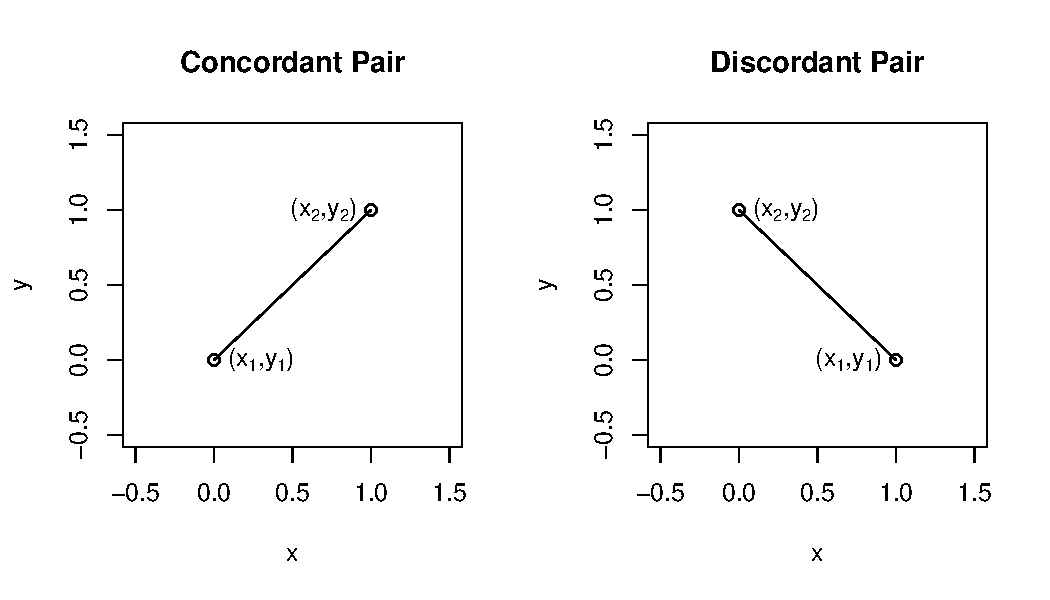
\includegraphics[scale=0.85]{images/pairs.pdf}
    %\caption{Two graphs showing examples of concordant and discordant pairs. Notice the plot to the right is increasing and the plot to the left is decreasing.}
    \caption{Two graphs showing examples of concordant and discordant pairs.}
    \label{fig:pairs}
\end{figure}
\begin{definition}\label{def:spearman_population}
    Consider a bivariate distribution with random pair $(X,Y)$. Let $(X_1,Y_1)$, $(X_2,Y_2)$, and $(X_3,Y_3)$ be independent and identically distributed pairs. Spearman's Rho of a population can be defined as $$\rho_S=3\left(P\left(\left(X_1-X_2\right)\left(Y_1-Y_3\right)>0\right)-P\left(\left(X_1-X_2\right)\left(Y_1-Y_3\right)<0\right)\right).$$
\end{definition}
It is important to notice the dependence between $X_1$  and $Y_1$ and the independence between $X_2$ and $Y_3$. The reason for this will become more clear in Section \ref{sec:modern_expressions}. Also note that the quantity in the parentheses is multiplied by 3. This is because the quantity inside ranges from $-\frac{1}{3}$ to $\frac{1}{3}$ (for detail see \cite{kruskal1958} p. 824). The first term in the parentheses is the probability of concordance and the second term is probability of discordance. Also notice that the second term is the compliment of the first. There are several ways to write Spearman's Rho by taking advantage of this result. We will see in Section \ref{sec:modern_expressions} that Spearman's Rho can be written in terms of probabilities, copulas, and CDFs. Although not obvious, we will later see how the sample definition and the population definition relate to each other.
%%%%%%%%%%%%%%%%%%%%%%%%%%%%%%%%%%%%%%%%%%%%%%%%%%%%%%%%%%%%%%%%%%%%%%%%%%%%%%%%%%%%%
%%%%%%%%%%%%%%%%%%%%%%%%%%%%%%%%%%%%%%%%%%%%%%%%%%%%%%%%%%%%%%%%%%%%%%%%%%%%%%%%%%%%%
%%%%%%%%%%%%%%%%%%%%%%%%%%%%%%%%%%%%%%%%%%%%%%%%%%%%%%%%%%%%%%%%%%%%%%%%%%%%%%%%%%%%%
%%%%%%%%%%%%%%%%%%%%%%%%%%%%%%%%%%%%%%%%%%%%%%%%%%%%%%%%%%%%%%%%%%%%%%%%%%%%%%%%%%%%%
%%%%%%%%%%%%%%%%%%%%%%%%%%%%%%%%%%%%%%%%%%%%%%%%%%%%%%%%%%%%%%%%%%%%%%%%%%%%%%%%%%%%%
\section{The History of Kendall's Tau}\label{sec:the_history_of_kendalls_tau}
\hspace{24pt} In 1938, the statistics community was introduced to Kendall's Tau ($\tau$), another measure of rank correlation \cite{kendall1938}. There are several parallels between Rho and Tau. They both have the ability to measure monotone behavior between two variables and also both require ranks to calculate. If both Rho and Tau are calculated on a set of data, often the quantities are relatively close, and usually the same sign. The idea of concordant and discordant pairs are used in the calculation of Tau.
\begin{definition}\label{def:kendalls_sample}
    Given a sample of raw data, $\left(x_1,y_1\right),\left(x_2,y_2\right),\ldots,\left(x_n,y_n\right)$, calculate the number of concordant pairs $c$ and number of discordant pairs $d$. Kendall's Tau of a sample can be defined as $$\widehat{\tau}=\frac{c-d}{c+d}=\frac{c-d}{{n \choose 2}}$$ where $n$ is the sample size.
\end{definition}
There is an alternate definition for both Rho and Tau that accounts for tied pairs, which is when the sign equals zero. Throughout the paper, continuous data will be studied. Therefore, the probability of a tie happening is zero. The alternative definitions of Tau can be useful for discrete data.

For the population definition we have to find the difference between the probability of concordance and the probability of discordance. Just like Rho, there will be several results that take advantage of the symmetry of the following definition.
\begin{definition}\label{def:kendalls_population}
    Consider a bivariate distribution with random pair $(X, Y)$. Let $(X_1,Y_1)$ and $(X_2,Y_2)$ be independent and identically distributed pairs. Kendall's Tau of a population can be defined as $$\tau=P\left(\left(X_1-X_2\right)\left(Y_1-Y_2\right)>0\right)-P\left(\left(X_1-X_2\right)\left(Y_1-Y_2\right)<0\right).$$
\end{definition}
This result looks intuitively symmetric and, much like Rho, we will define this quantity in Section \ref{sec:modern_expressions} in terms of probabilities, copulas, and CDFs. It is also important to notice the dependence between $X_1$ and $Y_1$, and the dependence between $X_2$ and $Y_2$.

Let's briefly relate this definition to the sample definition. Applying the Law of Large Numbers, think of the sample size approaching infinity. $$\lim_{n\to\infty}\frac{c-d}{{n \choose 2}}=\lim_{n\to\infty}\frac{c}{{n \choose 2}}-\lim_{n\to\infty}\frac{d}{{n \choose 2}}\longrightarrow \bigg(P\left(concordance\right)-P\left(discordance\right)\bigg)$$

This is a relaxed way to think about how the two definitions relate. To summarize, so far we have been introduced to the sample and population definitions of Spearman's Rho and Kendall's Tau.
%%%%%%%%%%%%%%%%%%%%%%%%%%%%%%%%%%%%%%%%%%%%%%%%%%%%%%%%%%%%%%%%%%%%%%%%%%%%%%%%%%%%%
%%%%%%%%%%%%%%%%%%%%%%%%%%%%%%%%%%%%%%%%%%%%%%%%%%%%%%%%%%%%%%%%%%%%%%%%%%%%%%%%%%%%%
%%%%%%%%%%%%%%%%%%%%%%%%%%%%%%%%%%%%%%%%%%%%%%%%%%%%%%%%%%%%%%%%%%%%%%%%%%%%%%%%%%%%%
%%%%%%%%%%%%%%%%%%%%%%%%%%%%%%%%%%%%%%%%%%%%%%%%%%%%%%%%%%%%%%%%%%%%%%%%%%%%%%%%%%%%%
%%%%%%%%%%%%%%%%%%%%%%%%%%%%%%%%%%%%%%%%%%%%%%%%%%%%%%%%%%%%%%%%%%%%%%%%%%%%%%%%%%%%%
\section{A General Case for Rank Correlation}\label{sec:general_coefficient}
\hspace{24pt} Apart from the correlation coefficients already introduced, in 1948 a general correlation coefficient was introduced by Maurice Kendall in his book {\it Rank Correlation Methods} \cite{kendall1990}. He proposed that this correlation coefficient is a generalization of coefficients such as Kendall's Tau ($\tau$), Spearman's Rho ($\rho_S$), and Pearson's Rho ($\rho$).
\begin{definition}\label{def:general_coefficient}
    To any pair of individuals, say the $i^{\text{th}}$ and the $j^{\text{th}}$, we will allot an $X$-score, denoted by $a_{ij}$, subject to the condition that $a_{ij}=-a_{ji}$. Similarly, we will allot a $Y$-score, denoted by $b_{ij}$, where $b_{ij}=-b_{ji}$. We define a generalized correlation coefficient $\Gamma$ by the equation $$\Gamma=\frac{\sum a_{ij}b_{ij}}{\sqrt{\left(\sum a_{ij}^2\sum b_{ij}^2\right)}}$$ and regard $a_{ij}$ as zero if $i=j$.
\end{definition}
We can define Kendall's Tau using this definition. Let $(X,Y)$ be a random bivariate vector with realized values $(x,y)$. Then let $r_i$ denote the rank of the $i^{\text{th}}$ object and $r_j$ denote the rank of the $j^{\text{th}}$ object, both ranked according to the variable $x$. Similarly, let $p_i$ denote the rank of the $i^{\text{th}}$ object and $p_j$ denote the rank of the $j^{\text{th}}$ object, both ranked according to the variable $y$. Define $$a_{ij}=\begin{cases}1 & ,r_i<r_j\\ -1 & ,r_i>r_j\\ \end{cases}$$ and $$b_{ij}=\begin{cases}1 & ,p_i<p_j\\ -1 & ,p_i>p_j\\ \end{cases}.$$ Using these parameters, Kendall's Tau is now defined in terms of the general correlation coefficient. Definition \ref{def:kendalls_sample} does not account for ties, but this general coefficient does. Because of this, the general coefficient is more powerful than the sample version. Again, our focus will be continuous data which has probability zero of a tie happening.

Spearman's Rho can be defined in a similar way. The parameters for Rho are much easier to implement. Using the same notation from the Tau case, define $$a_{ij}=r_j-r_i$$ and $$b_{ij}=p_j-p_i.$$ Spearman's Rho is now defined via parameters of the general correlation coefficient. It can easily be proved through algebraic manipulation that this way of defining it is equivalent to Definition \ref{def:spearman_sample}.

This general coefficient that Maurice Kendall discovered is a pleasing result. In addition to the similarities between the two rank correlation methods that we have already seen, there will be more parallels throughout the entirety of this paper.
%%%%%%%%%%%%%%%%%%%%%%%%%%%%%%%%%%%%%%%%%%%%%%%%%%%%%%%%%%%%%%%%%%%%%%%%%%%%%%%%%%%%%
%%%%%%%%%%%%%%%%%%%%%%%%%%%%%%%%%%%%%%%%%%%%%%%%%%%%%%%%%%%%%%%%%%%%%%%%%%%%%%%%%%%%%
%%%%%%%%%%%%%%%%%%%%%%%%%%%%%%%%%%%%%%%%%%%%%%%%%%%%%%%%%%%%%%%%%%%%%%%%%%%%%%%%%%%%%
%%%%%%%%%%%%%%%%%%%%%%%%%%%%%%%%%%%%%%%%%%%%%%%%%%%%%%%%%%%%%%%%%%%%%%%%%%%%%%%%%%%%%
%%%%%%%%%%%%%%%%%%%%%%%%%%%%%%%%%%%%%%%%%%%%%%%%%%%%%%%%%%%%%%%%%%%%%%%%%%%%%%%%%%%%%
\section{Modern Expressions for Rank Correlations}\label{sec:modern_expressions}
\hspace{24pt} Both of the population definitions we have seen for Rho and Tau have several equivalent forms, including in terms of copulas. Copulas are very important tools, as they are able to isolate information about the dependence structure of jointly distributed random variables. For the purposes of this project we only consider a bivariate case, but copulas can be extended to a $d$-dimensional case. We can define copulas more formally below, and follow with some related results and important theorems.
\begin{definition}\label{def:copula}
    A two-dimensional copula is a function $C:[0,1]^2\to [0,1]$ with bivariate inputs $(u,v)$ such that the following conditions are satisfied:
    \begin{enumerate}
        \item $C$ is a $2$-increasing function, the bivariate analog of a univariate non-decreasing function (for more detail, see \cite{nelsen2006} p. 8). Equivalently, for every $u_1,u_2,v_1,v_2\in[0,1]$ such that $u_1\leq u_2$ and $v_1\leq v_2$, $$C\left(u_2,v_2\right)-C\left(u_2,v_1\right)-C\left(u_1,v_2\right)+C\left(u_1,v_1\right)\geq 0.$$ This has also been called quasi-monotone \cite{scarsini1984}.
        \item $C\left(u,1\right)=u$ and $C\left(1,v\right)=v$.
        \item $C\left(u,0\right)=0$ and $C\left(0,v\right)=0$.
    \end{enumerate}
\end{definition}
\begin{definition}\label{def:pi}
    Let $\left(U,V\right)$ be a bivariate random vector with uniform marginals. An independence copulas is defined as $$\Pi\left(u,v\right)=uv.$$ In fact, random variables are independent if and only if their copula is the independence copula.
\end{definition}
The next Theorem (Sklar's) will allow us to use copulas in a practical manner. We incorporate CDFs and copulas so we can apply them to the definitions of Tau and Rho. Using the next Theorem we will be able to input marginal distributions for some arbitrary joint distribution function and output a quantity that can capture the dependence structure between each marginal distribution.
\begin{theorem}[Sklar's Theorem \cite{sklar1996}]\label{theorem:sklars}
    Let $F_{X,Y}\left(x,y\right)$ be a bivariate distribution function with marginals $F_X\left(x\right)$ and $F_Y\left(y\right)$. Then there exists a copula $C$ such that for all $\left(x,y\right)\in\mathbb{R}^2$, $$F_{X,Y}\left(x,y\right)=C\left(F_X\left(x\right),F_Y\left(y\right)\right).$$ If $F_X\left(x\right),F_Y\left(y\right)$ are continuous, then $C$ is unique; otherwise $C$ is uniquely determined on $\ran F_X\left(x\right)\times\ran F_Y\left(y\right)$. Conversely, if $C$ is a copula and $F_X\left(x\right),F_Y\left(y\right)$ are distribution functions, then the function $F_{X,Y}\left(x,y\right)$ defined above is a bivariate distribution function with marginals $F_X\left(x\right),F_Y\left(y\right)$.
\end{theorem}
\begin{corollary}\label{cor:sklars}
    Using the same notation as in Theorem \ref{theorem:sklars}, also let $F_X^{-1}\left(x\right)$ and $F_Y^{-1}\left(y\right)$ be quasi-inverses of $F_X\left(x\right)$ and $F_Y\left(y\right)$, respectively. Then for any $(u,v)\in\dom C$, $$C\left(u,v\right)=F_{X,Y}\left(F_X^{-1}\left(u\right),F_Y^{-1}\left(v\right)\right).$$
\end{corollary}
A quasi-inverse can be thought of as a traditional inverse function with weaker conditions. Now that we have defined copulas and how to apply copulas to probability distributions, we can harness their advantages and derive the rank correlation methods in terms of copulas. To assist in future calculation and notation, we will introduce the ``Q" construct. This will make the notation simpler.

The rest of the paper is scattered with a generalize integral of the form $$\int_a^bf\left(x\right)\mathrm{d}g\left(x\right).$$ This is called a Riemann-Steiljes integral, and by having the differential as a non-identity function it will essentially ``weight" the area of the curve with respect to the function $g\left(x\right)$. This idea can be extended into the bivariate case that we will utilize. This idea works when the function $g\left(x\right)$ satisfies general properties. However, when $g\left(x\right)$ does not satisfy these general properties, we will introduce a lemma that will fix that issue.
\begin{theorem}[The ``Q" Construct \cite{nelsen2006} p. 159]\label{theorem:Q}
     Let $\left(X_1,Y_1\right)$ and $\left(X_2,Y_2\right)$ be independent vectors of continuous random variables with joint distribution functions $F_1$ and $F_2$, respectively, with common marginals $F_X\left(x\right)$ and $F_Y\left(y\right)$. Let $C_1$ and $C_2$ denote the copulas of $\left(X_1,Y_1\right)$ and $\left(X_2,Y_2\right)$, respectively, so that $F_1\left(x,y\right)=C_1\left(F_X\left(x\right),F_Y\left(y\right)\right)$ and $F_2\left(x,y\right)=$ $C_2\left(F_X\left(x\right),F_Y\left(y\right)\right)$. Let $Q$ denote the difference between the probability of concordance and discordance of $\left(X_1,Y_1\right)$ and $\left(X_2,Y_2\right)$, i.e. let $$Q=P\left(\left(X_1-X_2\right)\left(Y_1-Y_2\right)>0\right)-P\left(\left(X_1-X_2\right)\left(Y_1-Y_2\right)<0\right).$$ Then $$Q=Q\left(C_1,C_2\right)=4\int\int_{[0,1]^2}C_2\left(u,v\right)\mathrm{d}C_1\left(u,v\right)-1.$$
\end{theorem}
\begin{proof}
    The random variables being used are continuous. Because of this, we can use the law of compliments to the following:
    \begin{align*}
        Q\left(C_1,C_2\right)&=P\left(\left(X_1-X_2\right)\left(Y_1-Y_2\right)>0\right)-P\left(\left(X_1-X_2\right)\left(Y_1-Y_2\right)<0\right)\\
        &=2P\left(\left(X_1-X_2\right)\left(Y_1-Y_2\right)>0\right)-1\\
        &=2\left[P\left(X_1>X_2,Y_1>Y_2\right)+P\left(X_2>X_1,Y_2>Y_1\right)\right]-1.
    \end{align*}
    It remains to show that 
    \begin{align*}
        P\left(X_1>X_2,Y_1>Y_2\right)+P\left(X_2>X_1,Y_2>Y_1\right)&=2P\left(X_1>X_2,Y_1>Y_2\right)\\
        &=2\int\int_{\mathbb{R}^2}C_2\left(u,v\right)\mathrm{d}C_1\left(u,v\right).
    \end{align*}
    We will spend the rest of the proof showing this. Start with the first term.
    \begin{align*}
        P\left(X_1>X_2,Y_1>Y_2\right)&=P\left(X_2<X_1,Y_2<Y_1\right)\\
        &=\int\int_{\mathbb{R}^2}P\left(X_2<x,Y_2<y\; |\; X_1=x,Y_1=y\right)f_1\left(x,y\right)\mathrm{d}x\mathrm{d}y\\
        &=\int\int_{\mathbb{R}^2}F_2\left(x,y\right)\mathrm{d}F_1\left(x,y\right)\\
        &=\int\int_{\mathbb{R}^2}C_2\left(F_X\left(x\right),F_Y\left(y\right)\right)\mathrm{d}C_1\left(F_X\left(x\right),F_Y\left(y\right)\right).
    \end{align*}
    The previous line invokes Sklar's Theorem. Using what we call a probability-integral transformation \cite{angus1994} we can introduce the transformations $u=F_X\left(x\right)$ and $v=F_Y\left(y\right)$. After applying the transformation, it follows that $$P\left(X_1>X_2,Y_1>Y_2\right)=\int\int_{[0,1]^2}C_2\left(u,v\right)\mathrm{d}C_1\left(u,v\right).$$
    Moving on to the second half of the proof, we will prove the next result. Let $S_i\left(x,y\right)$ be the survival function for the $i^{\text{th}}$ joint CDF.
    \begin{align*}
        P\left(X_1<X_2,Y_1<Y_2\right)&=P\left(X_2>X_1,Y_2>Y_1\right)\\
        &=\int\int_{\mathbb{R}^2}P\left(X_2>x,Y_2>y\; |\; X_1=x,Y_1=y\right)f_1\left(x,y\right)\mathrm{d}x\mathrm{d}y\\
        &=\int\int_{\mathbb{R}^2}S_2\left(x,y\right)\mathrm{d}F_1\left(x,y\right)\\
        &=\int\int_{\mathbb{R}^2}\left[1-F_X\left(x\right)-F_Y\left(y\right)+F_2\left(x,y\right)\right]\mathrm{d}F_1\left(x,y\right)\\
        &=\int\int_{\mathbb{R}^2}\left[1-F_X\left(x\right)-F_Y\left(y\right)+C_2\left(F_X\left(x\right),F_Y\left(y\right)\right)\right]\mathrm{d}C_1\left(F_X\left(x\right),F_Y\left(y\right)\right)
    \end{align*}
    The previous line invokes Sklar's Theorem. Using the same probability-integral transformation introduced earlier, it follows that
    \begin{align*}
        &=\int\int_{[0,1]^2}\left[1-u-v+C_2\left(u,v\right)\right]\mathrm{d}C_1\left(u,v\right)\\
        &=1-\frac{1}{2}-\frac{1}{2}+\int\int_{[0,1]^2}C_2\left(u,v\right)\mathrm{d}C_1\left(u,v\right)\\
        &=\int\int_{[0,1]^2}C_2\left(u,v\right)\mathrm{d}C_1\left(u,v\right).
    \end{align*}
    Thus, $$Q\left(C_2,C_1\right)=4\int\int_{[0,1]^2}C_2\left(u,v\right)\mathrm{d}C_1\left(u,v\right)-1.$$
\end{proof}
\begin{corollary}[``Q" corollary \cite{scarsini1984}]
    Using the same notation from Theorem \ref{theorem:Q}, also let $\overline{C}$ be a survival copula. A survival copula has the same properties as a typical survival function.
    \begin{enumerate}
        \item $Q$ is symmetric in its arguments. That is, $Q\left(C_1,C_2\right)=Q\left(C_2,C_1\right)$.
        \item Copulas can be replaced by survival copulas in $Q$. That is, $Q\left(C,\overline{C}\right)=Q\left(\overline{C},C\right)$.
    \end{enumerate}
\end{corollary}
With the help of all the previous definitions, theorems, and corollaries, we can define both Spearman's Rho and Kendall's Tau in terms of copulas. Along with each definition, we will have a short discussion about each rank correlation method. To overcome potential confusion, we will finally connect the sample definition and the population definition of Spearman's Rho, as we have already seen with Tau.
\begin{theorem}\label{theorem:rho}
     Let $\left(X,Y\right)$ be a continuous random vector and let $C$ be a copula for $\left(X,Y\right)$. Spearman's Rho can be defined as $$Q\left(C,\Pi\right)=12\int\int_{[0,1]^2}C\left(u,v\right)\mathrm{d}u\mathrm{d}v-3$$ where $\Pi$ is an independence copula.
\end{theorem}
\begin{proof}
    Recall from Definition \ref{def:spearman_population}, Spearman's Rho can be defined as $$\rho_S=3\left(P\left(\left(X_1-X_2\right)\left(Y_1-Y_3\right)>0\right)-P\left(\left(X_1-X_2\right)\left(Y_1-Y_3\right)<0\right)\right).$$ From Theorem \ref{theorem:Q}, we know the difference between the probability of concordance and discordance is the Q construct. The following form may appear different than Theorem \ref{theorem:Q}, but because $X_2$ and $Y_3$ are defined as independent, they will have an independence copula. Hence, $$\rho_S=3\left[4\int\int_{[0,1]^2}C\left(u,v\right)\mathrm{d}u\mathrm{d}v-1\right]=12\int\int_{[0,1]^2}C\left(u,v\right)\mathrm{d}u\mathrm{d}v-3=3Q\left(C,\Pi\right).$$
\end{proof}
An interesting result from the previous theorem can help us tie together the sample definition and the population version. It is important to restate that copulas of a probability distribution have uniform marginal distributions. Hence, $U\sim \text{Uni}\left(0,1\right)$ and $V\sim \text{Uni}\left(0,1\right)$. Note that the probability-integral transformation is used in the below derivation. Also recall the expected value and variance of a uniform distribution on $(0,1)$ are $\frac{1}{2}$ and $\frac{1}{12}$, respectively.
\begin{align*}
    \rho_S&=3Q\left(C,\Pi\right)\\
    &=12\int\int_{[0,1]^2}uv\mathrm{d}C\left(u,v\right)-3\\
    &=12\int\int_{[0,1]^2}uv\mathrm{d}F_{X,Y}\left(F_X^{-1}\left(u\right),F_Y^{-1}\left(v\right)\right)-3 &\text{(by Corollary \ref{cor:sklars})}\\
    &=12\int\int_{[0,1]^2}uv\mathrm{d}P\left(X<F_X^{-1}\left(u\right),Y<F_Y^{-1}\left(v\right)\right)-3\\
    &=12\int\int_{[0,1]^2}uv\mathrm{d}P\left(U<u,V<v\right)-3 &\text{(transformation)}\\
    &=12\int\int_{[0,1]^2}uvf_{U,V}\left(u,v\right)\mathrm{d}u\mathrm{d}v-3\\
    &=12\cdot \mathrm{E}\left[UV\right]-3\\
    &=\frac{\mathrm{E}\left[UV\right]-\frac{1}{4}}{\frac{1}{12}}\\
    &=\frac{\text{Cov}\left(U,V\right)}{\sqrt{\text{Var}\left(U\right)}\sqrt{\text{Var}\left(V\right)}}\\
    &=\rho\left(F_X\left(x\right),F_Y\left(y\right)\right).
\end{align*}
Even through the population definition in terms of copulas, we are still able to define it in terms of Pearson's correlation coefficient. In summary, the population version of Spearman's Rho is Pearson's evaluated in terms of the marginal CDFs.
\begin{theorem}\label{theorem:tau}
     Let $(X,Y)$ be a continuous random vector and let $C$ be a copula for $(X,Y)$. Kendall's Tau can be defined as $$Q\left(C,C\right)=4\int\int_{[0,1]^2}C\left(u.v\right)\mathrm{d}C\left(u,v\right)-1.$$
\end{theorem}
\begin{proof}
    Recall from Definition \ref{def:kendalls_population}, the population definition of Kendall's Tau is $$\tau=P\left(\left(X_1-X_2\right)\left(Y_1-Y_2\right)>0\right)-P\left(\left(X_1-X_2\right)\left(Y_1-Y_2\right)<0\right).$$ Apply Theorem \ref{theorem:Q} and we arrive at $$4\int\int_{[0,1]^2}C\left(u,v\right)\mathrm{d}C\left(u,v\right)-1=Q\left(C,C\right).$$
\end{proof}
Using the results from above, we can finally define both Spearman's Rho and Kendall's Tau in terms of CDFs. Although the bias that we will study in later sections can be achieved by using copulas, it is much easier to work with the definitions in terms of densities. The copulas will help during Chapter \ref{chap:MO} when we introduce the Marshall-Olkin distribution. The intuition behind the following theorem comes easily from the results above, so we will not prove them.
\begin{definition}\label{def:CDFexpressions}
    Let $\left(X,Y\right)$ be a continuous, random vector with joint CDF $F_{X,Y}\left(x,y\right)$ and respective marginals $F_X\left(x\right)$, $F_Y\left(y\right)$. We can define Spearman's Rho as $$\rho_S\left(X,Y\right)=12\int\int_{\mathbb{R}^2}F_{X,Y}\left(x,y\right)\mathrm{d}F_X\left(x\right)\mathrm{d}F_Y\left(y\right)-3$$ and Kendall's Tau as $$\tau\left(X,Y\right)=4\int\int_{\mathbb{R}^2}F_{X,Y}\left(x,y\right)\mathrm{d}F_{X,Y}\left(x,y\right)-1.$$
\end{definition}
\begin{proof}
    For both expression we will introduce the substitution $u=F_X\left(x\right)$ and $v=F_Y\left(y\right)$. Then, invoking Sklar's Theorem (\ref{theorem:sklars}) we get the following expressions.
    \begin{align*}
        \rho_S&=12\int\int_{[0,1]^2}C\left(u,v\right)\mathrm{d}u\mathrm{d}v-3\\
        &=12\int\int_{\mathbb{R}^2}F_{X,Y}\left(x,y\right)\mathrm{d}F_X\left(x\right)\mathrm{d}F_Y\left(y\right)-3\\[5mm]
        \tau&=4\int\int_{[0,1]^2}C\left(u,v\right)\mathrm{d}C\left(u,v\right)-1\\
        &=4\int\int_{\mathbb{R}^2}F_{X,Y}\left(x,y\right)\mathrm{d}F_{X,Y}\left(x,y\right)-1
    \end{align*}
\end{proof}
In summary, we can make the following observation. Ignoring the constants, Spearman's Rho can be defined as an integral over $\mathbb{R}^2$ of a joint CDF with respect to the two marginal CDFs. Similarly, ignoring the constants, Kendall's Tau can be defined as an integral over $\mathbb{R}^2$ of a joint CDF with respect to the joint CDF. Another way to think about these rank correlation methods is in terms of concordance and discordance. Ignoring constants, Spearman's Rho is the probability of concordance minus the probability of discordance, with the constraints that the marginals are independent. Similarly, ignoring the constants, Kendall's Tau is just the probability of concordance minus the probability of discordance.

In the next chapter we will see the expressions from Definition \ref{def:CDFexpressions} in terms of survival functions. The following lemma will show this is valid, and will also help simplify future calculations.
\begin{lemma}\label{lem:CDFsurvival}
    Let $F_{X,Y}\left(x,y\right)$ be a joint CDF with marginals joint densities $f_X\left(x\right)$ and $f_Y\left(y\right)$ with survival function $S_{X,Y}\left(x,y\right)$. Then $$\int\int_{\mathbb{R}^2}F_{X,Y}\left(x,y\right)\mathrm{d}F_X\left(x\right)\mathrm{d}F_Y\left(y\right)=\int\int_{\mathbb{R}^2}S_{X,Y}\left(x,y\right)\mathrm{d}S_X\left(x\right)\mathrm{d}S_{Y}\left(y\right)$$ and $$\int\int_{\mathbb{R}^2}F_{X,Y}\left(x,y\right)\mathrm{d}F_{X,Y}\left(x,y\right)=\int\int_{\mathbb{R}^2}S_{X,Y}\left(x,y\right)\mathrm{d}S_{X,Y}\left(x,y\right).$$
\end{lemma}
\begin{proof}
    Starting with the first expression,
    \begin{align*}
        &\int\int_{\mathbb{R}^2}F_{X,Y}\left(x,y\right)\mathrm{d}F_X\left(x\right)\mathrm{d}F_Y\left(y\right)\\
        =&\int\int_{\mathbb{R}^2}F_{X,Y}\left(x,y\right)f_X\left(x\right)f_Y\left(y\right)\mathrm{d}x\mathrm{d}y\\
        =&\int\int_{\mathbb{R}^2}\left[1-S_X\left(x\right)-S_Y\left(y\right)+S_{X,Y}\left(x,y\right)\right]f_X\left(x\right)f_Y\left(y\right)\mathrm{d}x\mathrm{d}y\\
        =&\int\int_{\mathbb{R}^2}\left[1-\left(1-F_X\left(x\right)\right)-\left(1-F_Y\left(y\right)\right)+S_{X,Y}\left(x,y\right)\right]f_X\left(x\right)f_Y\left(y\right)\mathrm{d}x\mathrm{d}y\\
        =&\int\int_{\mathbb{R}^2}f_X\left(x\right)f_Y\left(y\right)\mathrm{d}x\mathrm{d}y-\int\int_{\mathbb{R}^2}f_X\left(x\right)f_Y\left(y\right)\mathrm{d}x\mathrm{d}y-\int\int_{\mathbb{R}^2}f_X\left(x\right)f_Y\left(y\right)\mathrm{d}x\mathrm{d}y\\
        &+\int\int_{\mathbb{R}^2}F_X\left(x\right)f_X\left(x\right)f_Y\left(y\right)\mathrm{d}x\mathrm{d}y+\int\int_{\mathbb{R}^2}F_Y\left(y\right)f_X\left(x\right)f_Y\left(y\right)\mathrm{d}x\mathrm{d}y\\
        &+\int\int_{\mathbb{R}^2}S_{X,Y}\left(x,y\right)f_X\left(x\right)f_Y\left(y\right)\mathrm{d}x\mathrm{d}y
    \end{align*}
    Now introduce the substitutions $u=F_X\left(x\right)$ and $v=F_Y\left(y\right)$, where $\mathrm{d}u=f_X\left(x\right)\mathrm{d}x$ and $\mathrm{d}v=f_Y\left(y\right)\mathrm{d}y$.
    \begin{align*}
        =&-\int\int_{\mathbb{R}^2}f_X\left(x\right)f_Y\left(y\right)\mathrm{d}x\mathrm{d}y+\int_{\mathbb{R}}f_Y\left(y\right)\int_0^1u\mathrm{d}u\mathrm{d}y+\int_{\mathbb{R}}f_X\left(x\right)\int_0^1v\mathrm{d}v\mathrm{d}x\\
        &+\int\int_{\mathbb{R}^2}S_{X,Y}\left(x,y\right)f_X\left(x\right)f_Y\left(y\right)\mathrm{d}x\mathrm{d}y\\
        =&-1+\frac{1}{2}\int_{\mathbb{R}}f_Y\left(y\right)\mathrm{d}y+\frac{1}{2}\int_{\mathbb{R}}f_X\left(x\right)\mathrm{d}x+\int\int_{\mathbb{R}^2}S_{X,Y}\left(x,y\right)f_X\left(x\right)f_Y\left(y\right)\mathrm{d}x\mathrm{d}y\\
        =&-1+\frac{1}{2}+\frac{1}{2}+\int\int_{\mathbb{R}^2}S_{X,Y}\left(x,y\right)f_X\left(x\right)f_Y\left(y\right)\mathrm{d}x\mathrm{d}y\\
        =&\int\int_{\mathbb{R}^2}S_{X,Y}\left(x,y\right)f_X\left(x\right)f_Y\left(y\right)\mathrm{d}x\mathrm{d}y
    \end{align*}
    Now observe that $$\mathrm{d}S_X\left(x\right)\mathrm{d}S_Y\left(y\right)=\mathrm{d}\left(1-F_X\left(x\right)\right)\mathrm{d}\left(1-F_Y\left(y\right)\right)=f_X\left(x\right)f_Y\left(y\right)\mathrm{d}x\mathrm{d}y.$$ Hence, $$\int\int_{\mathbb{R}^2}F_{X,Y}\left(x,y\right)\mathrm{d}F_X\left(x\right)\mathrm{d}F_Y\left(y\right)=\int\int_{\mathbb{R}^2}S_{X,Y}\left(x,y\right)\mathrm{d}S_X\left(x\right)\mathrm{d}S_{Y}\left(y\right).$$
    The second expression is proved in a similar way.
    \begin{align*}
        &\int\int_{\mathbb{R}^2}F_{X,Y}\left(x,y\right)\mathrm{d}F_{X,Y}\left(x,y\right)\\
        =&\int\int_{\mathbb{R}^2}\left[1-S_X\left(x\right)-S_Y\left(y\right)+S_{X,Y}\left(x,y\right)\right]f_{X,Y}\left(x,y\right)\mathrm{d}x\mathrm{d}y\\
        =&\int\int_{\mathbb{R}^2}\left[1-\left(1-F_X\left(x\right)\right)-\left(1-F_Y\left(y\right)\right)+S_{X,Y}\left(x,y\right)\right]f_{X,Y}\left(x,y\right)\mathrm{d}x\mathrm{d}y\\
        =&\int\int_{\mathbb{R}^2}f_{X,Y}\left(x,y\right)\mathrm{d}x\mathrm{d}y-\int\int_{\mathbb{R}^2}f_{X,Y}\left(x,y\right)\mathrm{d}x\mathrm{d}y-\int\int_{\mathbb{R}^2}f_{X,Y}\left(x,y\right)\mathrm{d}x\mathrm{d}y\\
        &+\int\int_{\mathbb{R}^2}F_X\left(x\right)f_{X,Y}\left(x,y\right)\mathrm{d}x\mathrm{d}y+\int\int_{\mathbb{R}^2}F_Y\left(x\right)f_{X,Y}\left(x,y\right)\mathrm{d}x\mathrm{d}y\\
        &+\int\int_{\mathbb{R}^2}S_{X,Y}\left(x,y\right)f_{X,Y}\left(x,y\right)\mathrm{d}x\mathrm{d}y
    \end{align*}
    Now introduce the substitutions $u=F_X\left(x\right)$ and $v=F_Y\left(y\right)$, where $\mathrm{d}u=f_X\left(x\right)\mathrm{d}x$ and $\mathrm{d}v=f_Y\left(y\right)\mathrm{d}y$.
    \begin{align*}
        =&-\int\int_{\mathbb{R}^2}f_{X,Y}\left(x,y\right)+\int_{\mathbb{R}}f_{X,Y}\left(x,y\right)\int_0^1u\mathrm{d}u\mathrm{d}y+\int_{\mathbb{R}}f_{x,Y}\left(x,y\right)\int_0^1v\mathrm{d}v\mathrm{d}x\\
        &+\int\int_{\mathbb{R}^2}S_{X,Y}\left(x,y\right)f_{X,Y}\left(x,y\right)\mathrm{d}x\mathrm{d}y\\
        =&-1+\frac{1}{2}+\frac{1}{2}+\int\int_{\mathbb{R}^2}S_{x,Y}\left(x,y\right)f_{x,Y}\left(x,y\right)\mathrm{d}x\mathrm{d}y
    \end{align*}
    Now observe that $$\mathrm{d}S_{x,Y}\left(x,y\right)=\mathrm{d}\left(1-F_X\left(x\right)-F_Y\left(y\right)+F_{X,Y}\left(x,y\right)\right)=f_{X,Y}\left(x,y\right)\mathrm{d}x\mathrm{d}y.$$ Hence, $$\int\int_{\mathbb{R}^2}F_{X,Y}\left(x,y\right)\mathrm{d}F_{X,Y}\left(x,y\right)=\int\int_{\mathbb{R}^2}S_{X,Y}\left(x,y\right)\mathrm{d}S_{X,Y}\left(x,y\right).$$
\end{proof}
  \chapter{BIAS UNDER A MIXTURE MODEL AND ITS BEHAVIOR}\label{chap:bias_mixture}
%%%%%%%%%%%%%%%%%%%%%%%%%%%%%%%%%%%%%%%%%%%%%%%%%%%%%%%%%%%%%%%%%%%%%%%%%%%%%%%%%%%%%
%%%%%%%%%%%%%%%%%%%%%%%%%%%%%%%%%%%%%%%%%%%%%%%%%%%%%%%%%%%%%%%%%%%%%%%%%%%%%%%%%%%%%
%%%%%%%%%%%%%%%%%%%%%%%%%%%%%%%%%%%%%%%%%%%%%%%%%%%%%%%%%%%%%%%%%%%%%%%%%%%%%%%%%%%%%
%%%%%%%%%%%%%%%%%%%%%%%%%%%%%%%%%%%%%%%%%%%%%%%%%%%%%%%%%%%%%%%%%%%%%%%%%%%%%%%%%%%%%
%%%%%%%%%%%%%%%%%%%%%%%%%%%%%%%%%%%%%%%%%%%%%%%%%%%%%%%%%%%%%%%%%%%%%%%%%%%%%%%%%%%%%
\section{What Is a Mixture Model?}\label{sec:mixture_model}
\hspace{24pt} Mixture models can arise for multiple reasons. This could be due to bad sampling methods, diverse population, or it could be intended. In general, a mixture model represents a population with more than one distribution in it. For our purposes, we will be analyzing a bivariate mixture model that contains true, intended data, and contaminating, unwanted data. More formally, we can define a mixture model below.
\begin{definition}\label{def:mixture}
    Let $\vec{V}$ and $\vec{C}$ be bivariate random vectors from the valid distribution and contaminated distribution, respectively. Let $W\sim\text{Bernoulli}(p)$, where $p$ is the proportion of contamination. Then define a bivariate mixture model as $$\vec{M}=W\vec{C}+\left(1-W\right)\vec{V}.$$
\end{definition}
Consider the following scenario. Statisticians are collecting two statistics for undergraduate students at a university. They administer surveys randomly throughout campus without screening. There is a possibility that graduate students accidentally enter the sample unintended. Although the probability may be low, it still must be considered. This sample will contain a proportion ($p$) of unwanted, contaminated data. Assume that the distribution of each population is known where undergraduates are the valid data and the graduate students are the contaminating data, and $$\vec{V}\sim\text{Normal}\left(\vec{\mu} = \begin{bmatrix}0\\ 0\end{bmatrix},\;\Sigma = \begin{bmatrix}0.07 & -0.03\\ -0.03 & 0.05\end{bmatrix}\right)$$ $$\vec{C}\sim\text{Normal}\left(\vec{\mu} = \begin{bmatrix}2\\ 3 \end{bmatrix},\;\Sigma = \begin{bmatrix}0.03 & -0.05\\ -0.05 & 0.1\end{bmatrix}\right).$$ Taking a random sample from these populations and mixing accordingly, we can observe the results in Figure \ref{fig:mixPlots} below. In the first graph we are introducing no mixing, and is all the valid population. In the second graph there is half-valid, half-contaminated. The third graph contains all contaminated data, which would occur if the statistician samples the wrong population, entirely. This example of mixing illustrates the famous Simpson's Paradox. Notice the correlation is negative with no mixing, and as mixing is introduced the correlation becomes positive and then back to negative as the contamination takes over. This relationship between mixing and positive/negative correlation will be similar to the main results introduced throughout this chapter.
\begin{figure}[H]
    \centering
    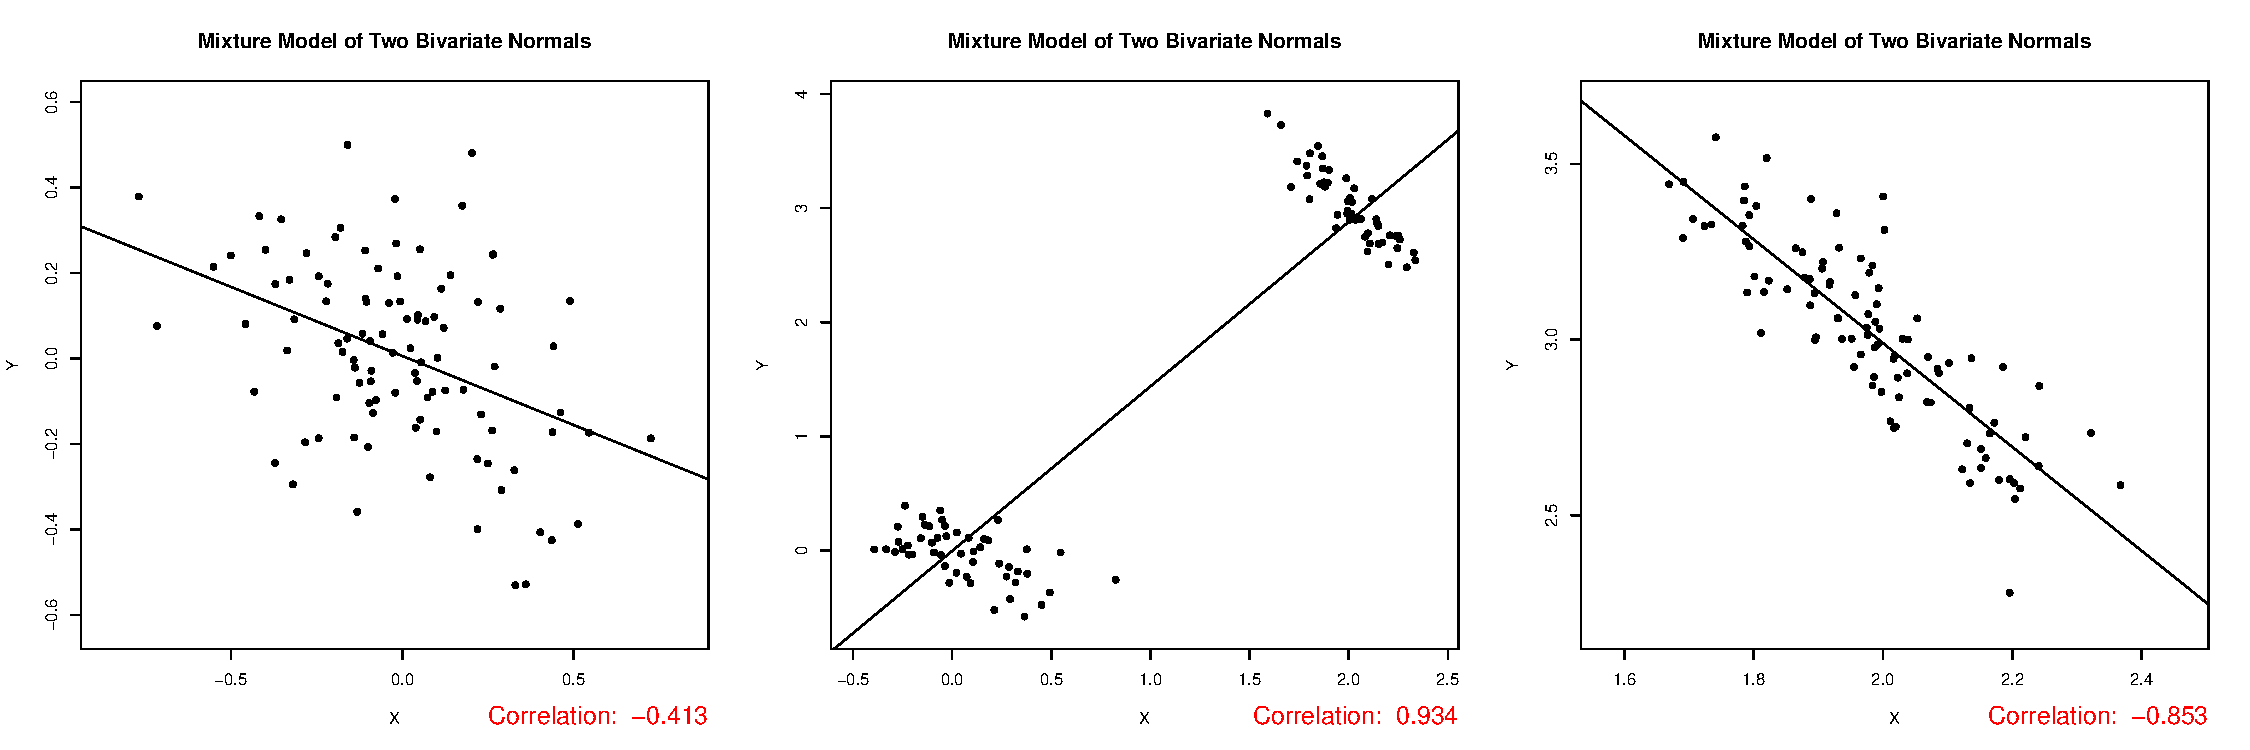
\includegraphics[scale=0.4]{images/mixturePlots.pdf}
    %\caption{Three different results of changing the mixing proportion ($p$). The first graph shows sampling the valid population. The second graph shows sampling half from the valid population and half from the contaminated population. The last graph shows sampling fully from the contaminated population. This diagram illustrates Simpson's Paradox. For visual convenience, the correlation is printed and the least-squares regression line is over-layed on each graph.}
    \caption{Three different results of changing the mixing proportion ($p$).}
    \label{fig:mixPlots}
\end{figure}
\hspace{24pt} The first graph shows sampling the valid population. The second graph shows sampling half from the valid population and half from the contaminated population. The last graph shows sampling fully from the contaminated population. This diagram illustrates Simpson's Paradox. For visual convenience, the correlation is printed and the least-squares regression line is over-layed on each graph.
%%%%%%%%%%%%%%%%%%%%%%%%%%%%%%%%%%%%%%%%%%%%%%%%%%%%%%%%%%%%%%%%%%%%%%%%%%%%%%%%%%%%%
%%%%%%%%%%%%%%%%%%%%%%%%%%%%%%%%%%%%%%%%%%%%%%%%%%%%%%%%%%%%%%%%%%%%%%%%%%%%%%%%%%%%%
%%%%%%%%%%%%%%%%%%%%%%%%%%%%%%%%%%%%%%%%%%%%%%%%%%%%%%%%%%%%%%%%%%%%%%%%%%%%%%%%%%%%%
%%%%%%%%%%%%%%%%%%%%%%%%%%%%%%%%%%%%%%%%%%%%%%%%%%%%%%%%%%%%%%%%%%%%%%%%%%%%%%%%%%%%%
%%%%%%%%%%%%%%%%%%%%%%%%%%%%%%%%%%%%%%%%%%%%%%%%%%%%%%%%%%%%%%%%%%%%%%%%%%%%%%%%%%%%%
\section{Bias Under Mixture Models}\label{sec:bias_mixtures}
\hspace{24pt} Traditionally, bias is defined as the difference between the expected value of an estimate and the true value of the parameter it is intended to estimate. In the context of Spearman's Rho, Kendall's Tau, and mixture models we define the bias as the difference between the parameter of the mixture and the parameter of the valid population. This can be defined more formally below.
\begin{definition}\label{def:bias_mixture}
    Let $\vec{V}$, $\vec{C}$, $\vec{M}$, $W$, and $p$ be described as in definition \ref{def:mixture}.  The bias under the mixture is
    \begin{align*}
        \text{Bias}_{\tau}(p)&=\tau_{\vec{M}}-\tau_{\vec{V}},\\
        \text{Bias}_{\rho}(p)&=\rho_{\vec{M}}-\rho_{\vec{V}}.
    \end{align*}
\end{definition}
Before the main result of the paper is introduced, there is one more lemma that will be used in the proof for Theorem \ref{theorem:main}. This lemma will use the property of the linearity of differentials and will help us prove later results.
\begin{lemma}\label{lem:differential}
    Let $f(x), g(x)$, and $h(x)$ be real-valued functions and let $a,b,c\in\mathbb{R}$. Then $$\int_s^t f(x)\mathrm{d}\left(ag(x)+bh(x)\right)=\int_s^t af(x)\mathrm{d}g(x)+\int_s^t bf(x)\mathrm{d}h(x).$$
\end{lemma}
Applying Definition \ref{def:bias_mixture} to the rank correlation methods, the main result of this paper can now be introduced.
\begin{theorem}\label{theorem:main}
    The bias in Kendall's Tau and Spearman's Rho due to mixing can be expressed as
    \begin{align*}
        \text{Bias}_{\tau}(p)&= 4\left(a_{\tau}p^2+b_{\tau}p\right)\\
        \text{Bias}_{\rho}(p)&= 12\left(a_{\rho}p^3+b_{\rho}p^2+c_{\rho}p\right),
    \end{align*}
    where
    \begin{align*}
        a_\tau=&\int\int_{\mathbb{R}^2}S_{\vec{V}}(x,y)\mathrm{d}S_{\vec{V}}(x,y)-\int\int_{\mathbb{R}^2}S_{\vec{V}}(x,y)\mathrm{d}S_{\vec{C}}(x,y)\\
        -&\int\int_{\mathbb{R}^2}S_{\vec{C}}(x,y)\mathrm{d}S_{\vec{V}}(x,y)+\int\int_{\mathbb{R}^2}S_{\vec{C}}(x,y)\mathrm{d}S_{\vec{C}}(x,y),\\
        b_\tau=&\int\int_{\mathbb{R}^2}S_{\vec{V}}(x,y)\mathrm{d}S_{\vec{C}}(x,y)+\int\int_{\mathbb{R}^2}S_{\vec{C}}(x,y)\mathrm{d}S_{\vec{V}}(x,y)\\
        -&2\int\int_{\mathbb{R}^2}S_{\vec{V}}(x,y)\mathrm{d}S_{\vec{V}}(x,y)
    \end{align*}
    and
    \begin{align*}
        a_\rho=&-\int\int_{\mathbb{R}^2}S_{\vec{V}}\left(x,y\right)\mathrm{d}S_{V_1}\left(x\right)\mathrm{d}S_{V_2}\left(y\right)+\int\int_{\mathbb{R}^2}S_{\vec{V}}\left(x,y\right)\mathrm{d}S_{V_1}\left(x\right)\mathrm{d}S_{C_2}\left(y\right)\\
        &+\int\int_{\mathbb{R}^2}S_{\vec{V}}\left(x,y\right)\mathrm{d}S_{C_1}\left(x\right)\mathrm{d}S_{V_2}\left(y\right)-\int\int_{\mathbb{R}^2}S_{\vec{V}}\left(x,y\right)\mathrm{d}S_{C_1}\left(x\right)\mathrm{d}S_{C_2}\left(y\right)\\
        &+\int\int_{\mathbb{R}^2}S_{\vec{C}}\left(x,y\right)\mathrm{d}S_{V_1}\left(x\right)\mathrm{d}S_{V_2}\left(y\right)-\int\int_{\mathbb{R}^2}S_{\vec{C}}\left(x,y\right)\mathrm{d}S_{V_1}\left(x\right)\mathrm{d}S_{C_2}\left(y\right)\\
        &-\int\int_{\mathbb{R}^2}S_{\vec{C}}\left(x,y\right)\mathrm{d}S_{C_1}\left(x\right)\mathrm{d}S_{V_2}\left(y\right)+\int\int_{\mathbb{R}^2}S_{\vec{C}}\left(x,y\right)\mathrm{d}S_{C_1}\left(x\right)\mathrm{d}S_{C_2}\left(y\right)\\
        b_\rho=&3\int\int_{\mathbb{R}^2}S_{\vec{V}}\left(x,y\right)\mathrm{d}S_{V_1}\left(x\right)\mathrm{d}S_{V_2}\left(y\right)-2\int\int_{\mathbb{R}^2}S_{\vec{V}}\left(x,y\right)\mathrm{d}S_{V_1}\left(x\right)\mathrm{d}S_{C_2}\left(y\right)\\
        &-2\int\int_{\mathbb{R}^2}S_{\vec{V}}\left(x,y\right)\mathrm{d}S_{C_1}\left(x\right)\mathrm{d}S_{V_2}\left(y\right)+\int\int_{\mathbb{R}^2}S_{\vec{V}}\left(x,y\right)\mathrm{d}S_{C_1}\left(x\right)\mathrm{d}S_{C_2}\left(y\right)\\
        &-2\int\int_{\mathbb{R}^2}S_{\vec{C}}\left(x,y\right)\mathrm{d}S_{V_1}\left(x\right)\mathrm{d}S_{V_2}\left(y\right)+\int\int_{\mathbb{R}^2}S_{\vec{C}}\left(x,y\right)\mathrm{d}S_{V_1}\left(x\right)\mathrm{d}S_{C_2}\left(y\right)\\
        &+\int\int_{\mathbb{R}^2}S_{\vec{C}}\left(x,y\right)\mathrm{d}S_{C_1}\left(x\right)\mathrm{d}S_{V_2}\left(y\right)\\
        c_\rho=&\int\int_{\mathbb{R}^2}S_{\vec{V}}\left(x,y\right)\mathrm{d}S_{V_1}\left(x\right)\mathrm{d}S_{C_2}\left(y\right)-3\int\int_{\mathbb{R}^2}S_{\vec{V}}\left(x,y\right)\mathrm{d}S_{V_1}\left(x\right)\mathrm{d}S_{V_2}\left(y\right)\\
        &+\int\int_{\mathbb{R}^2}S_{\vec{V}}\left(x,y\right)\mathrm{d}S_{C_1}\left(x\right)\mathrm{d}S_{V_2}\left(y\right)+\int\int_{\mathbb{R}^2}S_{\vec{C}}\left(x,y\right)\mathrm{d}S_{V_1}\left(x\right)\mathrm{d}S_{V_2}\left(y\right).
    \end{align*}
\end{theorem}
\begin{proof}
    Beginning with Kendall's Tau, we will start with the definition of bias.\\
    \begin{align*}
        \text{Bias}_{\tau}\left(p\right)=&\tau_{\vec{M}}-\tau_{\vec{V}}\\
        =&4\int\int_{\mathbb{R}^2}S_{\vec{M}}\left(x,y\right)\mathrm{d}S_{\vec{M}}\left(x,y\right)-1-\left(4\int\int_{\mathbb{R}^2}S_{\vec{V}}\left(x,y\right)\mathrm{d}S_{\vec{V}}\left(x,y\right)-1\right)\\
        =&4\int\int_{\mathbb{R}^2}\big[\left(1-p\right)S_{\vec{V}}\left(x,y\right)+pS_{\vec{C}}\left(x,y\right)\big]\mathrm{d}\left[\left(1-p\right)S_{\vec{V}}\left(x,y\right)+pS_{\vec{C}}\left(x,y\right)\right]\\
        &-4\int\int_{\mathbb{R}^2}S_{\vec{V}}\mathrm{d}S_{\vec{V}}\left(x,y\right).\\
    \end{align*}
    Now apply Lemma \ref{lem:differential}.
    \begin{align*}
        =&4\bigg[\int\int_{\mathbb{R}^2}\left(1-p\right)^2S_{\vec{V}}\left(x,y\right)\mathrm{d}S_{\vec{V}}\left(x,y\right)+\int\int_{\mathbb{R}^2}\left(1-p\right)pS_{\vec{V}}\left(x,y\right)\mathrm{d}S_{\vec{C}}\left(x,y\right)\\
        &+\int\int_{\mathbb{R}^2}p\left(1-p\right)S_{\vec{C}}\left(x,y\right)\mathrm{d}S_{\vec{V}}\left(x,y\right)+\int\int_{\mathbb{R}^2}p^2S_{\vec{C}}\left(x,y\right)\mathrm{d}S_{\vec{C}}\left(x,y\right)\bigg]\\
        &-4\int\int_{\mathbb{R}^2}S_{\vec{V}}\left(x,y\right)\mathrm{d}S_{\vec{V}}\left(x,y\right)\\
        =&4\bigg[\int\int_{\mathbb{R}^2}S_{\vec{V}}\left(x,y\right)\mathrm{d}S_{\vec{V}}\left(x,y\right)-2p\int\int_{\mathbb{R}^2}S_{\vec{V}}\left(x,y\right)\mathrm{d}S_{\vec{V}}\left(x,y\right)\\
        &+p^2\int\int_{\mathbb{R}^2}S_{\vec{V}}\left(x,y\right)\mathrm{d}S_{\vec{V}}\left(x,y\right)+p\int\int_{\mathbb{R}^2}S_{\vec{V}}\left(x,y\right)\mathrm{d}S_{\vec{C}}\left(x,y\right)\\
        &-p^2\int\int_{\mathbb{R}^2}S_{\vec{V}}\left(x,y\right)\mathrm{d}S_{\vec{C}}\left(x,y\right)+p\int\int_{\mathbb{R}^2}S_{\vec{C}}\left(x,y\right)\mathrm{d}S_{\vec{V}}\left(x,y\right)\\
        &-p^2\int\int_{\mathbb{R}^2}S_{\vec{C}}\left(x,y\right)\mathrm{d}S_{\vec{V}}\left(x,y\right)+p^2\int\int_{\mathbb{R}^2}S_{\vec{C}}\left(x,y\right)\mathrm{d}S_{\vec{C}}\left(x,y\right)\bigg]\\
        &-4\int\int_{\mathbb{R}^2}S_{\vec{V}}\left(x,y\right)\mathrm{d}S_{\vec{V}}\left(x,y\right)\\
        =&4\Bigg[p^2\bigg(\int\int_{\mathbb{R}^2}S_{\vec{V}}\left(x,y\right)\mathrm{d}S_{\vec{V}}\left(x,y\right)-\int\int_{\mathbb{R}^2}S_{\vec{V}}\left(x,y\right)\mathrm{d}S_{\vec{C}}\left(x,y\right)\\
        &-\int\int_{\mathbb{R}^2}S_{\vec{C}}\left(x,y\right)\mathrm{d}S_{\vec{V}}\left(x,y\right)+\int\int_{\mathbb{R}^2}S_{\vec{C}}\left(x,y\right)\mathrm{d}S_{\vec{C}}\left(x,y\right)\bigg)\\
        &+p\bigg(\int\int_{\mathbb{R}^2}S_{\vec{V}}\left(x,y\right)\mathrm{d}S_{\vec{C}}\left(x,y\right)+\int\int_{\mathbb{R}^2}S_{\vec{C}}\left(x,y\right)\mathrm{d}S_{\vec{V}}\left(x,y\right)\\
        &-2\int\int_{\mathbb{R}^2}S_{\vec{V}}\left(x,y\right)\mathrm{d}S_{\vec{V}}\left(x,y\right)\bigg)\Bigg]\\
        =&4\left(a_{\tau}p^2+b_{\tau}p\right).
    \end{align*}
    Using the same strategy above, we can use it solve for the bias of Rho under a mixture.
    \begin{align*}
        \text{Bias}_{\rho}\left(p\right)=&\rho_{\vec{M}}-\rho_{\vec{V}}\\
        =&12\int\int_{\mathbb{R}^2}S_{\vec{M}}\left(x,y\right)\mathrm{d}S_{M_1}\left(x\right)\mathrm{d}S_{M_2}\left(y\right)-3\\
        &-\left(12\int\int_{\mathbb{R}^2}S_{\vec{V}}\left(x,y\right)\mathrm{d}S_{V_1}\left(x\right)\mathrm{d}S_{V_2}\left(y\right)-3\right)\\
        =&12\int\int_{\mathbb{R}^2}\big[\left(1-p\right)S_{\vec{V}}\left(x,y\right)+pS_{\vec{C}}\left(x,y\right)\big]\\
        &\hspace{3cm}\mathrm{d}\big[\left(1-p\right)S_{V_1}\left(x\right)+pS_{C_1}\left(x\right)\big]\mathrm{d}\big[\left(1-p\right)S_{V_2}\left(y\right)+pS_{C_2}\left(y\right)\big]\\
        &-\left(12\int\int_{\mathbb{R}^2}S_{\vec{V}}\left(x,y\right)\mathrm{d}S_{V_1}\left(x\right)\mathrm{d}S_{V_2}\left(y\right)\right)\\
        =&12\bigg[\int\int_{\mathbb{R}^2}\left(1-p\right)^3S_{\vec{V}}\left(x,y\right)\mathrm{d}S_{V_1}\left(x\right)\mathrm{d}S_{V_2}\left(y\right)\\
        &+\int\int_{\mathbb{R}^2}\left(1-p\right)^2pS_{\vec{V}}\left(x,y\right)\mathrm{d}S_{V_1}\left(x\right)\mathrm{d}S_{C_2}\left(y\right)\\
        &+\int\int_{\mathbb{R}^2}\left(1-p\right)^2pS_{\vec{V}}\left(x,y\right)\mathrm{d}S_{C_1}\left(x\right)\mathrm{d}S_{V_2}\left(y\right)\\
        &+\int\int_{\mathbb{R}^2}\left(1-p\right)p^2S_{\vec{V}}\left(x,y\right)\mathrm{d}S_{C_1}\left(x\right)\mathrm{d}S_{C_2}\left(y\right)\\
        &+\int\int_{\mathbb{R}^2}\left(1-p\right)^2pS_{\vec{C}}\left(x,y\right)\mathrm{d}S_{V_1}\left(x\right)\mathrm{d}S_{V_2}\left(y\right)\\
        &+\int\int_{\mathbb{R}^2}p^2\left(1-p\right)S_{\vec{C}}\left(x,y\right)\mathrm{d}S_{V_1}\left(x\right)\mathrm{d}S_{C_2}\left(y\right)\\
        &+\int\int_{\mathbb{R}^2}p^2\left(1-p\right)S_{\vec{C}}\left(x,y\right)\mathrm{d}S_{C_1}\left(x\right)\mathrm{d}S_{V_2}\left(y\right)\\
        &+\int\int_{\mathbb{R}^2}p^3S_{\vec{C}}\left(x,y\right)\mathrm{d}S_{C_1}\left(x\right)\mathrm{d}S_{C_2}\left(y\right)\bigg]\\
        &-12\int\int_{\mathbb{R}^2}S_{\vec{V}}\left(x,y\right)\mathrm{d}S_{V_1}\left(x\right)\mathrm{d}S_{V_2}\left(y\right).
    \end{align*}
    \begin{align*}
        =&12\bigg[\int\int_{\mathbb{R}^2}S_{\vec{V}}\left(x,y\right)\mathrm{d}S_{V_1}\left(x\right)\mathrm{d}S_{V_2}\left(y\right)-3p\int\int_{\mathbb{R}^2}S_{\vec{V}}\left(x,y\right)\mathrm{d}S_{V_1}\left(x\right)\mathrm{d}S_{V_2}\left(y\right)\\
        &+3p^2\int\int_{\mathbb{R}^2}S_{\vec{V}}\left(x,y\right)\mathrm{d}S_{V_1}\left(x\right)\mathrm{d}S_{V_2}\left(y\right)-p^3\int\int_{\mathbb{R}^2}S_{\vec{V}}\left(x,y\right)\mathrm{d}S_{V_1}\left(x\right)\mathrm{d}S_{V_2}\left(y\right)\\
        &+p\int\int_{\mathbb{R}^2}S_{\vec{V}}\left(x,y\right)\mathrm{d}S_{V_1}\left(x\right)\mathrm{d}S_{C_2}\left(y\right)-2p^2\int\int_{\mathbb{R}^2}S_{\vec{V}}\left(x,y\right)\mathrm{d}S_{V_1}\left(x\right)\mathrm{d}S_{C_2}\left(y\right)\\
        &+p^3\int\int_{\mathbb{R}^2}S_{\vec{V}}\left(x,y\right)\mathrm{d}S_{V_1}\left(x\right)\mathrm{d}S_{C_2}\left(y\right)+p\int\int_{\mathbb{R}^2}S_{\vec{V}}\left(x,y\right)\mathrm{d}S_{C_1}\left(x\right)\mathrm{d}S_{V_2}\left(y\right)\\
        &-2p^2\int\int_{\mathbb{R}^2}S_{\vec{V}}\left(x,y\right)\mathrm{d}S_{C_1}\left(x\right)\mathrm{d}S_{V_2}\left(y\right)+p^3\int\int_{\mathbb{R}^2}S_{\vec{V}}\left(x,y\right)\mathrm{d}S_{C_1}\left(x\right)\mathrm{d}S_{V_2}\left(y\right)\\
        &+p^2\int\int_{\mathbb{R}^2}S_{\vec{V}}\left(x,y\right)\mathrm{d}S_{C_1}\left(x\right)\mathrm{d}S_{C_2}\left(y\right)-p^3\int\int_{\mathbb{R}^2}S_{\vec{V}}\left(x,y\right)\mathrm{d}S_{C_1}\left(x\right)\mathrm{d}S_{C_2}\left(y\right)\\
        &+p\int\int_{\mathbb{R}^2}S_{\vec{C}}\left(x,y\right)\mathrm{d}S_{V_1}\left(x\right)\mathrm{d}S_{V_2}\left(y\right)-2p^2\int\int_{\mathbb{R}^2}S_{\vec{C}}\left(x,y\right)\mathrm{d}S_{V_1}\left(x\right)\mathrm{d}S_{V_2}\left(y\right)\\
        &+p^3\int\int_{\mathbb{R}^2}S_{\vec{C}}\left(x,y\right)\mathrm{d}S_{V_1}\left(x\right)\mathrm{d}S_{V_2}\left(y\right)+p^2\int\int_{\mathbb{R}^2}S_{\vec{C}}\left(x,y\right)\mathrm{d}S_{V_1}\left(x\right)\mathrm{d}S_{C_2}\left(y\right)\\
        &-p^3\int\int_{\mathbb{R}^2}S_{\vec{C}}\left(x,y\right)\mathrm{d}S_{V_1}\left(x\right)\mathrm{d}S_{C_2}\left(y\right)+p^2\int\int_{\mathbb{R}^2}S_{\vec{C}}\left(x,y\right)\mathrm{d}S_{C_1}\left(x\right)\mathrm{d}S_{V_2}\left(Y\right)\\
        &-p^3\int\int_{\mathbb{R}^2}S_{\vec{C}}\left(x,y\right)\mathrm{d}S_{C_1}\left(x\right)\mathrm{d}S_{V_2}\left(y\right)+p^3\int\int_{\mathbb{R}^2}S_{\vec{C}}\left(x,y\right)\mathrm{d}S_{C_1}\left(x\right)\mathrm{d}S_{C_2}\left(y\right)\bigg]\\
        &-12\int\int_{\mathbb{R}^2}S_{\vec{V}}\left(x,y\right)\mathrm{d}S_{V_1}\left(x\right)\mathrm{d}S_{V_2}\left(y\right).
    \end{align*}
    \begin{align*}
        =&12\bigg[p^3\bigg(-\int\int_{\mathbb{R}^2}S_{\vec{V}}\left(x,y\right)\mathrm{d}S_{V_1}\left(x\right)\mathrm{d}S_{V_2}\left(y\right)+\int\int_{\mathbb{R}^2}S_{\vec{V}}\left(x,y\right)\mathrm{d}S_{V_1}\left(x\right)\mathrm{d}S_{C_2}\left(y\right)\\
        &+\int\int_{\mathbb{R}^2}S_{\vec{V}}\left(x,y\right)\mathrm{d}S_{C_1}\left(x\right)\mathrm{d}S_{V_2}\left(y\right)-\int\int_{\mathbb{R}^2}S_{\vec{V}}\left(x,y\right)\mathrm{d}S_{C_1}\left(x\right)\mathrm{d}S_{C_2}\left(y\right)\\
        &+\int\int_{\mathbb{R}^2}S_{\vec{C}}\left(x,y\right)\mathrm{d}S_{V_1}\left(x\right)\mathrm{d}S_{V_2}\left(y\right)-\int\int_{\mathbb{R}^2}S_{\vec{C}}\left(x,y\right)\mathrm{d}S_{V_1}\left(x\right)\mathrm{d}S_{C_2}\left(y\right)\\
        &-\int\int_{\mathbb{R}^2}S_{\vec{C}}\left(x,y\right)\mathrm{d}S_{C_1}\left(x\right)\mathrm{d}S_{V_2}\left(y\right)+\int\int_{\mathbb{R}^2}S_{\vec{C}}\left(x,y\right)\mathrm{d}S_{C_1}\left(x\right)\mathrm{d}S_{C_2}\left(y\right)\bigg)\\
        &+p^2\bigg(3\int\int_{\mathbb{R}^2}S_{\vec{V}}\left(x,y\right)\mathrm{d}S_{V_1}\left(x\right)\mathrm{d}S_{V_2}\left(y\right)-2\int\int_{\mathbb{R}^2}S_{\vec{V}}\left(x,y\right)\mathrm{d}S_{V_1}\left(x\right)\mathrm{d}S_{C_2}\left(y\right)\\
        &-2\int\int_{\mathbb{R}^2}S_{\vec{V}}\left(x,y\right)\mathrm{d}S_{C_1}\left(x\right)\mathrm{d}S_{V_2}\left(y\right)+\int\int_{\mathbb{R}^2}S_{\vec{V}}\left(x,y\right)\mathrm{d}S_{C_1}\left(x\right)\mathrm{d}S_{C_2}\left(y\right)\\
        &-2\int\int_{\mathbb{R}^2}S_{\vec{C}}\left(x,y\right)\mathrm{d}S_{V_1}\left(x\right)\mathrm{d}S_{V_2}\left(y\right)+\int\int_{\mathbb{R}^2}S_{\vec{C}}\left(x,y\right)\mathrm{d}S_{V_1}\left(x\right)\mathrm{d}S_{C_2}\left(y\right)\\
        &+\int\int_{\mathbb{R}^2}S_{\vec{C}}\left(x,y\right)\mathrm{d}S_{C_1}\left(x\right)\mathrm{d}S_{V_2}\left(y\right)\bigg)\\
        &+p\bigg(\int\int_{\mathbb{R}^2}S_{\vec{V}}\left(x,y\right)\mathrm{d}S_{V_1}\left(x\right)\mathrm{d}S_{C_2}\left(y\right)-3\int\int_{\mathbb{R}^2}S_{\vec{V}}\left(x,y\right)\mathrm{d}S_{V_1}\left(x\right)\mathrm{d}S_{V_2}\left(y\right)\\
        &+\int\int_{\mathbb{R}^2}S_{\vec{V}}\left(x,y\right)\mathrm{d}S_{C_1}\left(x\right)\mathrm{d}S_{V_2}\left(y\right)+\int\int_{\mathbb{R}^2}S_{\vec{C}}\left(x,y\right)\mathrm{d}S_{V_1}\left(x\right)\mathrm{d}S_{V_2}\left(y\right)\bigg)\bigg]\\
        =&12\left(a_{\rho}p^3+b_{\rho}p^2+c_{\rho}p\right).
    \end{align*}
\end{proof}
%%%%%%%%%%%%%%%%%%%%%%%%%%%%%%%%%%%%%%%%%%%%%%%%%%%%%%%%%%%%%%%%%%%%%%%%%%%%%%%%%%%%%
%%%%%%%%%%%%%%%%%%%%%%%%%%%%%%%%%%%%%%%%%%%%%%%%%%%%%%%%%%%%%%%%%%%%%%%%%%%%%%%%%%%%%
%%%%%%%%%%%%%%%%%%%%%%%%%%%%%%%%%%%%%%%%%%%%%%%%%%%%%%%%%%%%%%%%%%%%%%%%%%%%%%%%%%%%%
%%%%%%%%%%%%%%%%%%%%%%%%%%%%%%%%%%%%%%%%%%%%%%%%%%%%%%%%%%%%%%%%%%%%%%%%%%%%%%%%%%%%%
%%%%%%%%%%%%%%%%%%%%%%%%%%%%%%%%%%%%%%%%%%%%%%%%%%%%%%%%%%%%%%%%%%%%%%%%%%%%%%%%%%%%%
\section{General Behavior of Quadratics and Cubics}
\hspace{24pt} In the case of Tau, the final form expression for the bias is a quadratic without a constant term. In the case of Rho, the final form expression for the bias is a cubic without a constant term. For the interest of statistical application, it is common to want the sign of the bias. That is, whether the contamination will result in a positive or negative bias. By analyzing and characterizing all the different root behaviors, we can easily find the sign of the bias. Because the polynomials have no constant terms, our analysis will be simplified by having a root at zero.
\begin{prop}
    Consider a quadratic function without a constant term, $f(p)=ap^2+bp$. The following inequalities between $a$ and $b$ serve as a partition of the coefficient space that characterizes root behavior and thus the regions in the unit interval where the function is positive and negative. There are five cases below with subcases for some.
    \begin{enumerate}
        \item $f(p)=0$ for all $p$ in $(0,1)$. This occurs when $a=b=0$.
        \item $f(p)>0$ for all $p$ in $(0,1)$. This has two subcases.
        \begin{enumerate}
            \item $a\geq 0$ and $b\geq 0$ (but not both equal to zero).
            \item $0<-a\leq b$.
        \end{enumerate}
        \item $f(p)<0$ for all $p$ in $(0,1)$. This has two subcases.
        \begin{enumerate}
            \item $a\leq 0$ and $b\leq 0$ (but not both equal to zero).
            \item $b\leq -a<0$.
        \end{enumerate}
        \item There exists a root $p_1$ in $(0,1)$ such that $f(p)>0$ for $p<p_1$, but $f(p)<0$ for $p>p_1$.  This occurs when $0 < b < -a$. 
        \item There exists a non-zero root $p_1$ in $(0,1)$ such that $f(p) < 0$ for $p < p_1$, but $f(p) > 0$ for $p > p_1$.  This occurs when $-a < b < 0$.
    \end{enumerate}
    Consider a cubic function without a constant term, $f(p)=ap^3+bp^2 +cp$.  The following inequalities between $a,$ $b$, and $c$ serve as a partition of the coefficient space that characterizes root behavior and thus the regions in the unit interval where the function is positive and negative. There are 7 cases below with multiple subcases for some.
    \begin{enumerate}
        \item $f(p)=0$ for all $p$ in $(0,1)$. This occurs when $a=b=c=0$.
        \item $f(p)>0$ for all $p$ in $(0,1)$. This has four subcases.
        \begin{enumerate}
            \item $a>0$, $|b|<2\sqrt{ac}$, $c>0$.
            \item $a>0$, $|b|>2\sqrt{ac}$, $b\leq -2a$, $c\geq a$, $a+b+c\geq 0$.
            \item $a>0$, $b>0$, $c>0$, $|b|>2\sqrt{ac}$.
            \item $a<0$, $c>0$, $a+b+c\geq 0$.
        \end{enumerate}
        \item $f(p)<0$ for all $p$ in $(0,1)$. This has four subcases.
        \begin{enumerate}
            \item $a<0$, $|b|<2\sqrt{ac}$, $c<0$.
            \item $a<0$, $|b|>2\sqrt{ac}$, $b\geq -2a$, $c\leq a$, $a+b+c\leq 0$.
            \item $a<0$, $b<0$, $c<0$, $|b|>2\sqrt{ac}$.
            \item $a>0$, $c<0$, $a+b+c\leq 0$.
        \end{enumerate}
        \item There exists a non-zero root $p_1$ in $(0,1)$ such that $f(p)>0$ for $p<p_1$, but $f(p)<0$ for $p>p_1$. This has two subcases.
        \begin{enumerate}
            \item $a>0$, $b\leq -a$, $c>0$, $|b|>2\sqrt{ac}$, $a+b+c\leq0$.
            \item $a<0$, $c>0$, $a+b+c\leq 0$.
        \end{enumerate}
        \item There exists a non-zero root $p_1$ in $(0,1)$ such that $f(p)<0$ for $0<p<p_1$, but $f(p)>0$ for $p_1<p<1$. This has two subcases.
        \begin{enumerate}
            \item $a<0$, $b\geq -a$, $c<0$, $|b|>2\sqrt{ac}$, $a+b+c\geq 0$.
            \item $a>0$, $c<0$, $a+b+c\geq 0$.
        \end{enumerate}
        \item There exists two non-zero roots $p_1<p_2$ in $(0,1)$ such that $f(p)>0$ for $0<p<p_1$, $f(p)<0$ for $p_1<p<p_2$, and $f(p)>0$ for $p_2<p<1$. This occurs when $a>0$, $-2a\leq b\leq 0$, $c\leq a$, $|b|>2\sqrt{ac}$, $a+b+c\geq0$.
        \item There exists two non-zero roots $p_1<p_2$ in $(0,1)$ such that $f(p)<0$ for $0<p<p_1$, $f(p)>0$ for $p_1<p<p_2$, and $f(p)<0$ for $p_2<p<1$. This occurs when $a<0$, $-2a\geq b\geq 0$, $c\geq a$, $|b|>2\sqrt{ac}$, $a+b+c\leq 0$.
    \end{enumerate}
\end{prop}
The proof of these cases are elementary, yet tedious, and will be skipped. The application of these cases will be shown graphically in Chapter \ref{chap:MO} when we study the Marshall-Olkin distribution.
  \chapter{THE MARSHALL-OLKIN DISTRIBUTION}\label{chap:MO}
%%%%%%%%%%%%%%%%%%%%%%%%%%%%%%%%%%%%%%%%%%%%%%%%%%%%%%%%%%%%%%%%%%%%%%%%%%%%%%%%%%%%%
%%%%%%%%%%%%%%%%%%%%%%%%%%%%%%%%%%%%%%%%%%%%%%%%%%%%%%%%%%%%%%%%%%%%%%%%%%%%%%%%%%%%%
%%%%%%%%%%%%%%%%%%%%%%%%%%%%%%%%%%%%%%%%%%%%%%%%%%%%%%%%%%%%%%%%%%%%%%%%%%%%%%%%%%%%%
%%%%%%%%%%%%%%%%%%%%%%%%%%%%%%%%%%%%%%%%%%%%%%%%%%%%%%%%%%%%%%%%%%%%%%%%%%%%%%%%%%%%%
%%%%%%%%%%%%%%%%%%%%%%%%%%%%%%%%%%%%%%%%%%%%%%%%%%%%%%%%%%%%%%%%%%%%%%%%%%%%%%%%%%%%%
\section{Introducing the Marshall-Olkin Distribution}
\hspace{24pt} Albert W. Marshall and Ingram Olkin introduced the Marshall-Olkin (MO) distribution in 1967. They claimed that they were the first to have proposed a multivariate exponential distribution with an applicable use. This distribution arises from ``shock models" and its ability to model the failing of a two-component system \cite{marshallolkin1967}. Define three independent random variables, where $Z_1\sim\text{Exp}\left(\lambda_1\right)$, $Z_2\sim\text{Exp}\left(\lambda_2\right)$, and $Z_3\sim\text{Exp}\left(\lambda_3\right)$ represent the time until occurrences of the shocks. The first two random variables are shocks to component one and component two, respectively, and the last random variable is a shock to both components. Now define two random variables $X=\min\{Z_1,Z_3\}$ and $Y=\min\{Z_2,Z_3\}$. These new random variables represent the lifetimes of component one and component two, respectively. We can now find the joint survival function. The survival function will allow for more convenient calculations than working with the joint CDF.
\begin{align*}
    S_{X,Y}\left(x,y\right)&=P\left(X>x,Y>y\right)\\
    &=P\left(\min\{Z_1,Z_3\}>x,\min\{Z_2,Z_3\}>y\right)\\
    &=P\left(Z_1>x,Z_3>x,Z_2>y,Z_3>y\right)\\
    &=P\left(Z_1>x,Z_2>y,Z_3>\max\{x,y\}\right)\\
    &=\exp\left\{-\left(\lambda_1x+\lambda_2y+\lambda_3\max\{x,y\}\right)\right\},\qquad x,y>0
\end{align*}
The visual of an exponential distribution curve is very well known. However, the MO distribution is difficult to visualize because of the ``max" term. Let's show an example with three different sets of parameters.
\begin{figure}[ht]
    \centering
    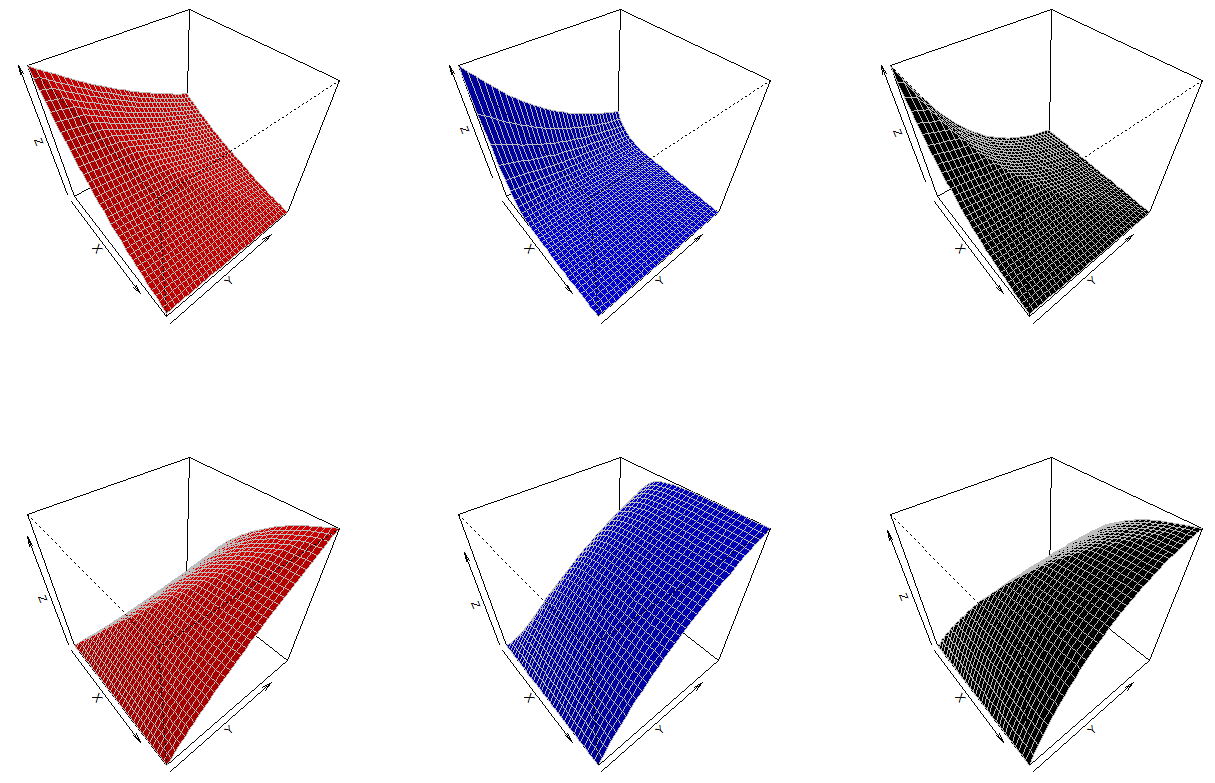
\includegraphics[scale=0.45]{images/3DMO.PNG}
    %\caption{The red graph shows $\lambda_1=1$, $\lambda_2=0.2$, and $\lambda_3=0.5$. The blue graph shows $\lambda_1=10$, $\lambda_2=1$, and $\lambda_3=0.5$. The black graph shows $\lambda_1,=0.5$, $\lambda_2=0.5$, $\lambda_3=2$. The top row shows the survival function and the bottom row shows the CDF.}
    \caption{The red graph shows $\lambda_1=1$, $\lambda_2=0.2$, and $\lambda_3=0.5$; the blue graph shows $\lambda_1=10$, $\lambda_2=1$, and $\lambda_3=0.5$; the black graph shows $\lambda_1,=0.5$, $\lambda_2=0.5$, $\lambda_3=2$; the top row shows the survival function and the bottom row shows the CDF.}
    \label{fig:MO3d}
\end{figure}
%%%%%%%%%%%%%%%%%%%%%%%%%%%%%%%%%%%%%%%%%%%%%%%%%%%%%%%%%%%%%%%%%%%%%%%%%%%%%%%%%%%%%
%%%%%%%%%%%%%%%%%%%%%%%%%%%%%%%%%%%%%%%%%%%%%%%%%%%%%%%%%%%%%%%%%%%%%%%%%%%%%%%%%%%%%
%%%%%%%%%%%%%%%%%%%%%%%%%%%%%%%%%%%%%%%%%%%%%%%%%%%%%%%%%%%%%%%%%%%%%%%%%%%%%%%%%%%%%
%%%%%%%%%%%%%%%%%%%%%%%%%%%%%%%%%%%%%%%%%%%%%%%%%%%%%%%%%%%%%%%%%%%%%%%%%%%%%%%%%%%%%
%%%%%%%%%%%%%%%%%%%%%%%%%%%%%%%%%%%%%%%%%%%%%%%%%%%%%%%%%%%%%%%%%%%%%%%%%%%%%%%%%%%%%
\section{Rank Correlation of the Marshall-Olkin Distribution}
\hspace{24pt} The population definitions have been defined in multiple ways for both Spearman's Rho and Kendall's Tau. We can now use them to define these rank correlation methods for the MO distribution. We will begin with Spearman's Rho, because for Kendall's Tau we have to invoke a Lemma that will be defined soon.
\begin{theorem}\label{theorem:MOrho}
    Spearman's Rho for the Marshall-Olkin distribution can be defined as $$\rho_S=\frac{3\alpha_1\alpha_2}{2\alpha_1+2\alpha_2-\alpha_1\alpha_2}$$ where $\alpha_1=\frac{\lambda_3}{\lambda_1+\lambda_3}$ and $\alpha=\frac{\lambda_3}{\lambda_2+\lambda_3}$.
\end{theorem}
\begin{proof}
    Recall Theorem \ref{theorem:rho}, where Spearman's Rho is defined as $$Q\left(C,\Pi\right)=12\int\int_{[0,1]^2}C\left(u,v\right)\mathrm{d}u\mathrm{d}v-3.$$ We can use this definition by finding the copula for the MO distribution. To find the copula, make the following observations. Notice that $\max\left\{x,y\right\}=x+y-\min\left\{x,y\right\}$. The marginal survival functions for $X$ and $Y$ are $S_X\left(x\right)=\exp\left\{-\left(\lambda_1+\lambda_3\right)x\right\}$ and $S_Y\left(y\right)=\exp\left\{-\left(\lambda_2+\lambda_3\right)y\right\}$, respectively. To make future calculations easier, let $\alpha_1=\frac{\lambda_3}{\lambda_1+\lambda_3}$ and $\alpha_2=\frac{\lambda_3}{\lambda_2+\lambda_3}$. Using these observations, we will start with the survival function, manipulate it, then apply the copula transformation.
    \begin{align*}
        S_{X,Y}\left(x,y\right)&=\exp\left\{-\left(\lambda_1x+\lambda_2y+\lambda_3\max\left\{x,y\right\}\right)\right\}\\
        &=\exp\left\{-\left(\lambda_1+\lambda_3\right)x-\left(\lambda_2+\lambda_3\right)y+\lambda_3\min\left\{x,y\right\}\right\}\\
        &=\exp\left\{-\left(\lambda_1+\lambda_3\right) x\right\}\exp\left\{-\left(\lambda_2+\lambda_3\right)y\right\}\exp\left\{\lambda_3\min\left\{x,y\right\}\right\}\\
        &=S_X\left(x\right)S_Y\left(y\right)\min\left\{\exp\left\{\lambda_3x\right\},\;\exp\left\{\lambda_3y\right\}\right\}
    \end{align*}
    Using the fact that $\exp\left\{\lambda_3x\right\}=S_X\left(x\right)^{-\alpha_1}$ and $\exp\left\{\lambda_3y\right\}=S_Y\left(y\right)^{-\alpha_2}$, now apply the copula transformation $U=F_X\left(x\right)$, $V=F_Y\left(y\right)$. Let $\overline{C}$ be the survival copula.
    \begin{align*}
        \overline{C}\left(u,v\right)&=u\, v\min\left\{u^{-\alpha_1},v^{-\alpha_2}\right\}\\
        &=\min\left\{v\, u^{1-\alpha_1},u\, v^{1-\alpha_2}\right\}\\
        &=\begin{cases}v\, u^{1-\alpha_1} & ,u^{\alpha_1}\geq v^{\alpha_2}\\ u\, v^{1-\alpha_2} & ,u^{\alpha_1}\leq v^{\alpha_2}\\ \end{cases}
    \end{align*}
    The MO distribution contains a singular component. This is a concentrated cluster of density on the line $y=x$ (or the line $u^{\alpha_1}=v^{\alpha_2}$). Because of this, the integral in Theorem \ref{theorem:rho} will have to be split into two parts to account for this cluster. To visualize this, consider Figure \ref{fig:MOsim} below, a simulation done using the software R. Now that the copula has been defined, apply to Theorem \ref{theorem:rho}.
    \begin{figure}
        \centering
        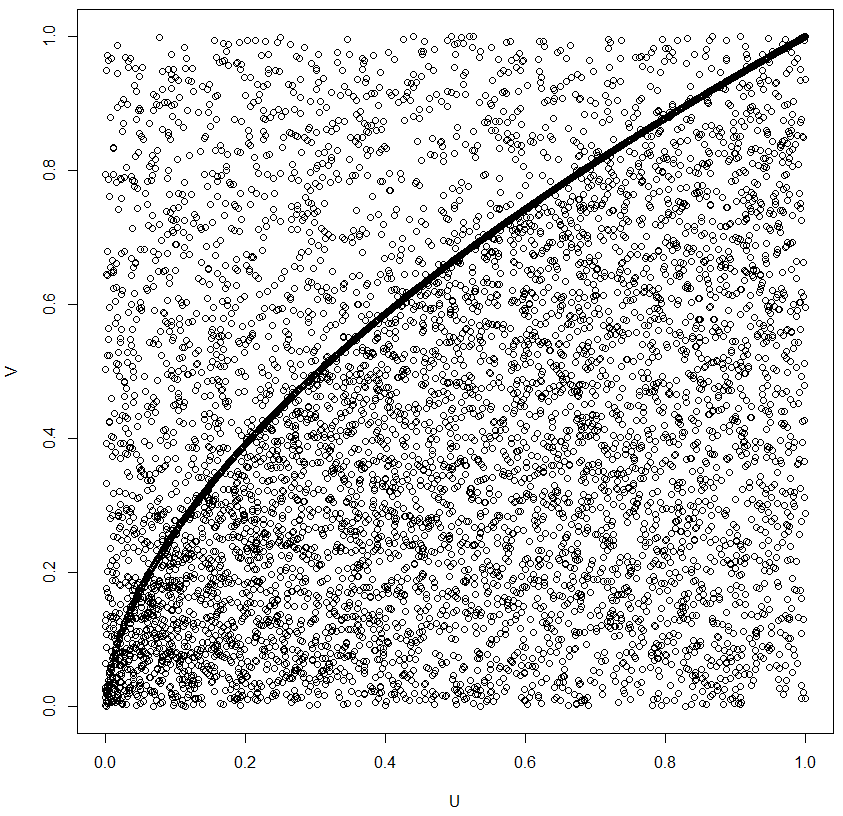
\includegraphics[scale=0.6]{images/MOsimulation.PNG}
        %\caption{Simulation of the Marshall-Olkin survival copula using parameters: $\lambda_1=0.7$, $\lambda_2=0.2$, and $\lambda_3=0.5$. The simulation is done in the open-source software R.}
        \caption{Simulation of the Marshall-Olkin survival copula using parameters: $\lambda_1=0.7$, $\lambda_2=0.2$, and $\lambda_3=0.5$.}
        \label{fig:MOsim}
    \end{figure}
    \begin{align*}
        \rho_S&=12\int\int_{[0,1]^2}C\left(u,v\right)\mathrm{d}u\mathrm{d}v-3\\
        &=12\int_0^1\left[\int_0^{u^{\alpha_1/\alpha_2}}v\, u^{1-\alpha_1}\mathrm{d}v+\int_{u^{\alpha_1/\alpha_2}}^1u\, v^{1-\alpha_2}\mathrm{d}v\right]\mathrm{d}u-3\\
        &=12\int_0^1\left[u^{1-\alpha_1}\frac{1}{2}v^2\bigg|_0^{u^{\alpha_1/\alpha_2}}+u\, \frac{v^{2-\alpha_2}}{2-\alpha_2}\bigg|_{u^{\alpha_1/\alpha_2}}^1\right]\mathrm{d}u-3\\
        &=12\int_0^1\left[\frac{u^{1-\alpha_1}u^{2\alpha_1/\alpha_2}}{2}+\left(\frac{u}{2-\alpha_2}-\frac{u\, u^{\left(\alpha_1/\alpha_2\right)\left(2-\alpha_2\right)}}{2-\alpha_2}\right)\right]\mathrm{d}u-3\\
        &=12\int_0^1\left[u^{2\alpha_1/\alpha_2-\alpha_1+1}\left(\frac{1}{2}-\frac{1}{2-\alpha_2}\right)+\frac{u}{2-\alpha_2}\right]\mathrm{d}u-3\\
        &=12\left[\left(\frac{1}{2}-\frac{1}{2-\alpha_2}\right)\frac{u^{2\alpha_1/\alpha_2-\alpha_1+2}}{2\alpha_1/\alpha_2-\alpha_1+2}\bigg|_0^1+\frac{u^2}{2\left(2-\alpha_2\right)}\bigg|_0^1\right]-3\\
        &=12\left[\left(\frac{1}{2}-\frac{1}{2-\alpha_2}\right)\left(\frac{1}{2\alpha_1/\alpha_2-\alpha_1+2}\right)+\frac{1}{2\left(2-\alpha_2\right)}\right]-3\\
        &=12\left[\frac{2-\alpha_2-2+2\alpha_1/\alpha_2-\alpha_1+2}{2\left(2-\alpha_2\right)\left(2\alpha_1/\alpha_2-\alpha_1+2\right)}\right]-3\\
        &=\frac{-12\alpha_2+24\alpha_1/\alpha_2-12\alpha_1+24}{2\left(2-\alpha_2\right)\left(2\alpha_1/\alpha_2-\alpha_1+2\right)}-\frac{6\left(2-\alpha_2\right)\left(2\alpha_1\alpha_2-\alpha_1+2\right)}{2\left(2-\alpha_2\right)\left(2\alpha_1/\alpha_2-\alpha_1+2\right)}\\
        &=\frac{12\alpha_1-6\alpha_1\alpha_2}{2\left(2-\alpha_2\right)\left(2\alpha_1/\alpha_2-\alpha_1+2\right)}\\
        &=\frac{3\alpha_1}{2\alpha_1/\alpha_2-\alpha_1+2}\\
        &=\frac{3\alpha_1\alpha_2}{2\alpha_1+2\alpha_2-\alpha_1\alpha_2}
    \end{align*}
    In terms of lambda, we can define it as $$\rho_S=\frac{3\left(\frac{\lambda_3}{\lambda_1+\lambda_3}\right)\left(\frac{\lambda_3}{\lambda_2+\lambda_3}\right)}{2\left(\frac{\lambda_3}{\lambda_1+\lambda_3}\right)+2\left(\frac{\lambda_3}{\lambda_2+\lambda_3}\right)-\left(\frac{\lambda_3}{\lambda_1+\lambda_3}\right)\left(\frac{\lambda_3}{\lambda_2+\lambda_3}\right)}$$
\end{proof}
For the Kendall's Tau definition of the MO distribution, we will take the same route as Spearman's Rho by using the copula. We will first define a lemma to help us evaluate integrals with singular components. The original lemma was proved by Li, X. in 2002 \cite{li2002} in terms of copulas. Here, we state it in terms of CDFs.
\begin{lemma}\label{lem:li}
    Let $F_{X,Y}\left(x,y\right)$ and $G_{X,Y}\left(x,y\right)$ be differentiable CDFs. Then $$\int\int_{\mathbb{R}^2}F_{X,Y}\left(x,y\right)\mathrm{d}G_{X,Y}\left(x,y\right)=\frac{1}{2}-\int\int_{\mathbb{R}^2}\frac{\partial}{\partial x}F_{X,Y}\left(x,y\right)\frac{\partial}{\partial y}G_{X,Y}\left(x,y\right)\mathrm{d}x\mathrm{d}y.$$
\end{lemma}
Using Lemma \ref{lem:li}, we will now derive Kendall's Tau for the MO distribution.
\begin{theorem}\label{theorem:MOtau}
    Kendall's Tau for the Marshall-Olkin distribution can be derived as $$\tau=\frac{\alpha_1\alpha_2}{\alpha_1+\alpha_2-\alpha_1\alpha_2}$$ where $\alpha_1=\frac{\lambda_3}{\lambda_1+\lambda_3}$ and $\alpha=\frac{\lambda_3}{\lambda_2+\lambda_3}$.
\end{theorem}
\begin{proof}
    \begin{align*}
        \tau&=4\int\int_{[0,1]^2}C\left(u,v\right)\mathrm{d}C\left(u,v\right)-1\\
        &=4\left[\frac{1}{2}-\int\int_{[0,1]^2}\frac{\partial}{\partial u}C\left(u,v\right)\frac{\partial}{\partial v}C\left(u,v\right)\mathrm{d}u\mathrm{d}v\right]-1\\
        &=4\left[\frac{1}{2}-\int_0^1\left(\int_0^{u^{\alpha_1/\alpha_2}}\frac{\partial}{\partial u}u^{1-\alpha_1}v\frac{\partial}{\partial v}u^{1-\alpha_1}v\mathrm{d}v+\int_{u^{\alpha_1/\alpha_2}}^1\frac{\partial}{\partial u}uv^{1-\alpha_2}\frac{\partial}{\partial v}uv^{1-\alpha_2}\mathrm{d}v\right)\mathrm{d}u\right]-1\\
        &=4\left[\frac{1}{2}-\int_0^1\left(\int_0^{u^{\alpha_1/\alpha_2}}\left(1-\alpha_1\right)u^{-\alpha_1}vu^{1-\alpha_1}\mathrm{d}v-\int_{u^{\alpha_1/\alpha_2}}^1uv^{1-\alpha_2}\left(1-\alpha_2\right)v^{-\alpha_2}\mathrm{d}v\right)\mathrm{d}u\right]-1\\
        &=4\left[\frac{1}{2}-\int_0^1\left(\frac{1-\alpha_1}{2}u^{1-2\alpha_1}v^2\bigg|_0^{u^{\alpha_1/\alpha_2}}+\frac{1-\alpha_2}{2-2\alpha_2}uv^{2-2\alpha_2}\bigg|_{u^{\alpha_1/\alpha_2}}^1\right)\mathrm{d}u\right]-1\\
        &=4\left[\frac{1}{2}-\int_0^1\left(\frac{1-\alpha_1}{2}u^{2\alpha_1/\alpha_2-2\alpha_1+1}+\frac{1}{2}u-\frac{1}{2}u^{2\alpha_1/\alpha_2-2\alpha_1+1}\right)\mathrm{d}u\right]-1\\
        &=2\left(1+\alpha_1\frac{u^{2\alpha_1/\alpha_2-2\alpha_1+2}}{2\alpha_1/\alpha_2-2\alpha_1+2}\bigg|_0^1-\frac{1}{2}u^2\bigg|_0^1\right)-1\\
        &=2\left(1+\frac{\alpha_1}{2\alpha_1/\alpha_2-2\alpha_1+2}-\frac{1}{2}\right)-1\\
        &=\frac{\alpha_1}{\alpha_1/\alpha_2-\alpha_1+1}\\
        &=\frac{\alpha_1\alpha_2}{\alpha_1+\alpha_2-\alpha_1\alpha_2}
    \end{align*}
    In terms of lambda, we can define it as $$\tau=\frac{\left(\frac{\lambda_3}{\lambda_1+\lambda_3}\right)\left(\frac{\lambda_3}{\lambda_2+\lambda_3}\right)}{\frac{\lambda_3}{\lambda_1+\lambda_3}+\frac{\lambda_3}{\lambda_2+\lambda_3}+\left(\frac{\lambda_3}{\lambda_1+\lambda_3}\right)\left(\frac{\lambda_3}{\lambda_2+\lambda_3}\right)}$$
\end{proof}
For both of the previous proofs we could have arrived at the same solutions by using the CDF versions. We now have all the information we need to find the bias of the Marshall-Olkin distribution in terms of the mixing proportion, $p$.
%%%%%%%%%%%%%%%%%%%%%%%%%%%%%%%%%%%%%%%%%%%%%%%%%%%%%%%%%%%%%%%%%%%%%%%%%%%%%%%%%%%%%
%%%%%%%%%%%%%%%%%%%%%%%%%%%%%%%%%%%%%%%%%%%%%%%%%%%%%%%%%%%%%%%%%%%%%%%%%%%%%%%%%%%%%
%%%%%%%%%%%%%%%%%%%%%%%%%%%%%%%%%%%%%%%%%%%%%%%%%%%%%%%%%%%%%%%%%%%%%%%%%%%%%%%%%%%%%
%%%%%%%%%%%%%%%%%%%%%%%%%%%%%%%%%%%%%%%%%%%%%%%%%%%%%%%%%%%%%%%%%%%%%%%%%%%%%%%%%%%%%
%%%%%%%%%%%%%%%%%%%%%%%%%%%%%%%%%%%%%%%%%%%%%%%%%%%%%%%%%%%%%%%%%%%%%%%%%%%%%%%%%%%%%
\section{Bias of Rank Correlation Under a Mixture Model}\label{sec:MObias}
\hspace{24pt} Consider two populations that follow a bivariate Marshall-Olkin distribution, one being a valid population and the other contaminating. Define the parameters for each to be $$\left(X,Y\right)_V\sim\text{MO}\left(\lambda_{V1},\lambda_{V2},\lambda_{V3}\right)\qquad\text{and}\qquad\left(X,Y\right)_C\sim\text{MO}\left(\lambda_{C1},\lambda_{C2},\lambda_{C3}\right).$$
To find the bias in terms of the mixing proportion we can anticipate there will be a lot of integrals to solve in order to arrive at the desired analytical solution. However, by noticing a pattern for each integral in the coefficients from Theorem \ref{theorem:main} we can formulate a general integral to solve. This is because each integral follows a similar form, the only difference being valid or contaminated survival function. Furthermore, some of the integrals are equivalent to the ones solved in both Theorem \ref{theorem:MOrho} and \ref{theorem:MOtau}. Recall the bias from Theorem \ref{theorem:main}, $$\text{Bias}_{\tau}\left(p\right)=\tau_{\vec{M}}-\tau_{\vec{V}}=4\left(a_{\tau}p^2+b_{\tau}p\right)$$ where
\begin{align*}
    a_\tau=&\int\int_{\mathbb{R}^2}S_{\vec{V}}(x,y)\mathrm{d}S_{\vec{V}}(x,y)-\int\int_{\mathbb{R}^2}S_{\vec{V}}(x,y)\mathrm{d}S_{\vec{C}}(x,y)\\
    -&\int\int_{\mathbb{R}^2}S_{\vec{C}}(x,y)\mathrm{d}S_{\vec{V}}(x,y)+\int\int_{\mathbb{R}^2}S_{\vec{C}}(x,y)\mathrm{d}S_{\vec{C}}(x,y),\\
    b_\tau=&\int\int_{\mathbb{R}^2}S_{\vec{V}}(x,y)\mathrm{d}S_{\vec{C}}(x,y)+\int\int_{\mathbb{R}^2}S_{\vec{C}}(x,y)\mathrm{d}S_{\vec{V}}(x,y)\\
    -&2\int\int_{\mathbb{R}^2}S_{\vec{V}}(x,y)\mathrm{d}S_{\vec{V}}(x,y).
\end{align*}
\hspace{24pt} In the coefficients above, there are four unique integrals. Instead of solving all four integrals directly, we can solve a general integral. Beginning with the bias for Tau, we will generalize the integral using placeholder parameters, $(\alpha_1,\alpha_2,\alpha_3)$ and $\left(\beta_1,\beta_2,\beta_3\right)$. Think of these as being the valid and contaminated parameters, allowing us to rearrange them without loss of generality.
\begin{align*}
    &\int\int_{\mathbb{R}^2}S_{\alpha}\left(x,y\right)\mathrm{d}S_{\beta}\left(x,y\right)\\
    =&\int_0^{\infty}\int_0^{\infty}e^{-\alpha_1x-\alpha_2y-\alpha_3\max\left\{x,y\right\}}\mathrm{d}e^{-\beta_1x-\beta_2y-\beta_3\max\left\{x,y\right\}}\\
    =&\frac{1}{2}-\int_0^{\infty}\int_0^{\infty}\frac{\partial}{\partial x}e^{-\alpha_1x-\alpha_2y-\alpha_3\max\left\{x,y\right\}}\frac{\partial}{\partial y}e^{-\beta_1x-\beta_2y-\beta_3\max\left\{x,y\right\}}\mathrm{d}x\mathrm{d}y\\
    =&\frac{1}{2}-\int_0^{\infty}\int_y^{\infty}\left(\alpha_1+\alpha_3\right)\beta_2e^{-\left(\alpha_1+\alpha_3+\beta_1+\beta_3\right)x-\left(\alpha_2+\beta_2\right)y}\mathrm{d}x\mathrm{d}y\\
    &\hspace{3.5mm}-\int_0^{\infty}\int_x^{\infty}\alpha_1\left(\beta_2+\beta_3\right)e^{-\left(\alpha_1+\beta_1\right)x-\left(\alpha_2+\alpha_3+\beta_2+\beta_3\right)y}\mathrm{d}y\mathrm{d}x\\
    =&\frac{1}{2}+\int_0^{\infty}\left[\frac{\left(\alpha_1+\alpha_3\right)\beta_2}{\alpha_1+\alpha_3+\beta_1+\beta_3}e^{-\left(\alpha_1+\alpha_3+\beta_1+\beta_3\right)x-\left(\alpha_2+\beta_2\right)y}\bigg|_y^{\infty}\right]\mathrm{d}y\\
    &\hspace{3.5mm}+\int_0^{\infty}\left[\frac{\alpha_1\left(\beta_2+\beta_3\right)}{\alpha_2+\alpha_3+\beta_2+\beta_3}e^{-\left(\alpha_1+\beta_1\right)x-\left(\alpha_2+\alpha_3+\beta_2+\beta_3\right)y}\bigg|_x^{\infty}\right]\mathrm{d}x\\
    =&\frac{1}{2}-\frac{\left(\alpha_1+\alpha_3\right)\beta_2}{\alpha_1+\alpha_3+\beta_1+\beta_3}\int_0^{\infty}e^{-\left(\alpha_1+\alpha_2+\alpha_3+\beta_1+\beta_2+\beta_3\right)y}\mathrm{d}y\\
    &\hspace{3.5mm}-\frac{\alpha_1\left(\beta_2+\beta_3\right)}{\alpha_2+\alpha_3+\beta_2+\beta_3}\int_0^{\infty}e^{-\left(\alpha_1+\alpha_2+\alpha_3+\beta_1+\beta_2+\beta_3\right)x}\mathrm{d}x\\
    =&\frac{1}{2}-\frac{\left(\alpha_1+\alpha_3\right)\beta_2}{\alpha_1+\alpha_3+\beta_1+\beta_3}\left(\frac{-1}{\alpha_1+\alpha_2+\alpha_3+\beta_1+\beta_2+\beta_3}e^{-\left(\alpha_1+\alpha_2+\alpha_3+\beta_1+\beta_2+\beta_3\right)y}\bigg|_0^{\infty}\right)\\
    &\hspace{3.5mm}-\frac{\alpha_1\left(\beta_2+\beta_3\right)}{\alpha_2+\alpha_3+\beta_2+\beta_3}\left(\frac{-1}{\alpha_1+\alpha_2+\alpha_3+\beta_1+\beta_2+\beta_3}e^{-\left(\alpha_1+\alpha_2+\alpha_3+\beta_1+\beta_2+\beta_3\right)x}\bigg|_0^{\infty}\right)\\
    =&\frac{1}{2}-\frac{1}{\alpha_1+\alpha_2+\alpha_3+\beta_1+\beta_2+\beta_3}\left(\frac{\left(\alpha_1+\alpha_3\right)\beta_2}{\alpha_1+\alpha_3+\beta_1+\beta_3}+\frac{\alpha_1\left(\beta_2+\beta_3\right)}{\alpha_2+\alpha_3+\beta_2+\beta_3}\right)
\end{align*}
Observe that if the survival functions are the same for both the integrand and the differential, the general solution reduces to the form $$\int\int_{\mathbb{R}^2}S_{\alpha}\left(x,y\right)\mathrm{d}S_{\alpha}\left(x,y\right)=\frac{1}{2}-\frac{\alpha_1+\alpha_2}{4\alpha_1+4\alpha_2+4\alpha_3}.$$
Now that the general integral is solved, the last step is to plug in the correct parameters for each corresponding integral. The coefficients for the bias of Tau can be defined as
{\footnotesize
\begin{align*}
    a_{\tau}=&\frac{1}{2}-\frac{\lambda_{V1}+\lambda_{V2}}{4\lambda_{V1}+4\lambda_{V2}+4\lambda_{V3}}\\
    &-\left(\frac{1}{2}-\frac{1}{\lambda_{V1}+\lambda_{V2}+\lambda_{V3}+\lambda_{C1}+\lambda_{C2}+\lambda_{C3}}\left(\frac{\left(\lambda_{V1}+\lambda_{V3}\right)\lambda_{C2}}{\lambda_{V1}+\lambda_{V3}+\lambda_{C1}+\lambda_{C3}}+\frac{\lambda_{V1}\left(\lambda_{V2}+\lambda_{V3}\right)}{\lambda_{V2}+\lambda_{V3}+\lambda_{C2}+\lambda_{C3}}\right)\right)\\
    &-\left(\frac{1}{2}-\frac{1}{\lambda_{C1}+\lambda_{C2}+\lambda_{C3}+\lambda_{V1}+\lambda_{V2}+\lambda_{V3}}\left(\frac{\left(\lambda_{C1}+\lambda_{C3}\right)\lambda_{V2}}{\lambda_{C1}+\lambda_{C3}+\lambda_{V1}+\lambda_{V3}}+\frac{\lambda_{C1}\left(\lambda_{C2}+\lambda_{C3}\right)}{\lambda_{C2}+\lambda_{C3}+\lambda_{V2}+\lambda_{V3}}\right)\right)\\
    &+\frac{1}{2}-\frac{\lambda_{C1}+\lambda_{C2}}{4\lambda_{C1}+4\lambda_{C2}+4\lambda_{C3}}\\
    b_{\tau}=&\left(\frac{1}{2}-\frac{1}{\lambda_{V1}+\lambda_{V2}+\lambda_{V3}+\lambda_{C1}+\lambda_{C2}+\lambda_{C3}}\left(\frac{\left(\lambda_{V1}+\lambda_{V3}\right)\lambda_{C2}}{\lambda_{V1}+\lambda_{V3}+\lambda_{C1}+\lambda_{C3}}+\frac{\lambda_{V1}\left(\lambda_{V2}+\lambda_{V3}\right)}{\lambda_{V2}+\lambda_{V3}+\lambda_{C2}+\lambda_{C3}}\right)\right)\\
    &+\left(\frac{1}{2}-\frac{1}{\lambda_{C1}+\lambda_{C2}+\lambda_{C3}+\lambda_{V1}+\lambda_{V2}+\lambda_{V3}}\left(\frac{\left(\lambda_{C1}+\lambda_{C3}\right)\lambda_{V2}}{\lambda_{C1}+\lambda_{C3}+\lambda_{V1}+\lambda_{V3}}+\frac{\lambda_{C1}\left(\lambda_{C2}+\lambda_{C3}\right)}{\lambda_{C2}+\lambda_{C3}+\lambda_{V2}+\lambda_{V3}}\right)\right)\\
    &-2\left(\frac{1}{2}-\frac{\lambda_{V1}+\lambda_{V2}}{4\lambda_{V1}+4\lambda_{V2}+4\lambda_{V3}}\right).
\end{align*}}
After elementary algebra steps we can arrive at the final expression for the coefficients for the bias of Tau as
{\footnotesize
\begin{align*}
    a_{\tau}=&\frac{1}{\lambda_{V1}+\lambda_{V2}+\lambda_{V3}+\lambda_{C1}+\lambda_{C2}+\lambda_{C3}}\\
    &\hspace{2cm}\cdot\left(\frac{\left(\lambda_{V1}+\lambda_{V3}\right)\lambda_{C2}+\left(\lambda_{C1}+\lambda_{C3}\right)\lambda_{V2}}{\lambda_{V1}+\lambda_{V3}+\lambda_{C1}+\lambda_{C3}}+\frac{\lambda_{V1}\left(\lambda_{V2}+\lambda_{V3}\right)+\lambda_{C1}\left(\lambda_{C2}+\lambda_{C3}\right)}{\lambda_{V2}+\lambda_{V3}+\lambda_{C2}+\lambda_{C3}}\right)\\
    &-\left(\frac{\lambda_{V1}+\lambda_{V2}}{4\lambda_{V1}+4\lambda_{V2}+4\lambda_{V3}}+\frac{\lambda_{C1}+\lambda_{C2}}{4\lambda_{C1}+4\lambda_{C2}+4\lambda_{C3}}\right)\\
    b_{\tau}=&\frac{\lambda_{V1}+\lambda_{V2}}{2\lambda_{V1}+2\lambda_{V2}+2\lambda_{V3}}\\        &-\frac{1}{\lambda_{V1}+\lambda_{V2}+\lambda_{V3}+\lambda_{C1}+\lambda_{C2}+\lambda_{C3}}\\
    &\hspace{2cm}\cdot\left(\frac{\left(\lambda_{V1}+\lambda_{V3}\right)\lambda_{C2}+\left(\lambda_{C1}+\lambda_{C3}\right)\lambda_{V2}}{\lambda_{V1}+\lambda_{V3}+\lambda_{C1}+\lambda_{C3}}+\frac{\lambda_{V1}\left(\lambda_{V2}+\lambda_{V3}\right)+\lambda_{C1}\left(\lambda_{C2}+\lambda_{C3}\right)}{\lambda_{V2}+\lambda_{V3}+\lambda_{C2}+\lambda_{C3}}\right).
\end{align*}}
Solving for the coefficient for the bias of Rho is achieved following the same process. There are eight unique integrals in the case of Rho, so we will also solve a general integral. Recall the bias from Theorem \ref{theorem:main}, $$\text{Bias}_{\rho}(p)=\rho_{\vec{M}}-\rho_{\vec{V}}=12\left(a_{\rho}p^3+b_{\rho}p^2+c_{\rho}p\right)$$ where
\begin{align*}
    a_\rho=&-\int\int_{\mathbb{R}^2}S_{\vec{V}}\left(x,y\right)\mathrm{d}S_{V_1}\left(x\right)\mathrm{d}S_{V_2}\left(y\right)+\int\int_{\mathbb{R}^2}S_{\vec{V}}\left(x,y\right)\mathrm{d}S_{V_1}\left(x\right)\mathrm{d}S_{C_2}\left(y\right)\\
    &+\int\int_{\mathbb{R}^2}S_{\vec{V}}\left(x,y\right)\mathrm{d}S_{C_1}\left(x\right)\mathrm{d}S_{V_2}\left(y\right)-\int\int_{\mathbb{R}^2}S_{\vec{V}}\left(x,y\right)\mathrm{d}S_{C_1}\left(x\right)\mathrm{d}S_{C_2}\left(y\right)\\
    &+\int\int_{\mathbb{R}^2}S_{\vec{C}}\left(x,y\right)\mathrm{d}S_{V_1}\left(x\right)\mathrm{d}S_{V_2}\left(y\right)-\int\int_{\mathbb{R}^2}S_{\vec{C}}\left(x,y\right)\mathrm{d}S_{V_1}\left(x\right)\mathrm{d}S_{C_2}\left(y\right)\\
    &-\int\int_{\mathbb{R}^2}S_{\vec{C}}\left(x,y\right)\mathrm{d}S_{C_1}\left(x\right)\mathrm{d}S_{V_2}\left(y\right)+\int\int_{\mathbb{R}^2}S_{\vec{C}}\left(x,y\right)\mathrm{d}S_{C_1}\left(x\right)\mathrm{d}S_{C_2}\left(y\right)\\
    b_\rho=&3\int\int_{\mathbb{R}^2}S_{\vec{V}}\left(x,y\right)\mathrm{d}S_{V_1}\left(x\right)\mathrm{d}S_{V_2}\left(y\right)-2\int\int_{\mathbb{R}^2}S_{\vec{V}}\left(x,y\right)\mathrm{d}S_{V_1}\left(x\right)\mathrm{d}S_{C_2}\left(y\right)\\
    &-2\int\int_{\mathbb{R}^2}S_{\vec{V}}\left(x,y\right)\mathrm{d}S_{C_1}\left(x\right)\mathrm{d}S_{V_2}\left(y\right)+\int\int_{\mathbb{R}^2}S_{\vec{V}}\left(x,y\right)\mathrm{d}S_{C_1}\left(x\right)\mathrm{d}S_{C_2}\left(y\right)\\
    &-2\int\int_{\mathbb{R}^2}S_{\vec{C}}\left(x,y\right)\mathrm{d}S_{V_1}\left(x\right)\mathrm{d}S_{V_2}\left(y\right)+\int\int_{\mathbb{R}^2}S_{\vec{C}}\left(x,y\right)\mathrm{d}S_{V_1}\left(x\right)\mathrm{d}S_{C_2}\left(y\right)\\
    &+\int\int_{\mathbb{R}^2}S_{\vec{C}}\left(x,y\right)\mathrm{d}S_{C_1}\left(x\right)\mathrm{d}S_{V_2}\left(y\right)\\
    c_\rho=&-3\int\int_{\mathbb{R}^2}S_{\vec{V}}\left(x,y\right)\mathrm{d}S_{V_1}\left(x\right)\mathrm{d}S_{V_2}\left(y\right)+\int\int_{\mathbb{R}^2}S_{\vec{V}}\left(x,y\right)\mathrm{d}S_{V_1}\left(x\right)\mathrm{d}S_{C_2}\left(y\right)\\
    &+\int\int_{\mathbb{R}^2}S_{\vec{V}}\left(x,y\right)\mathrm{d}S_{C_1}\left(x\right)\mathrm{d}S_{V_2}\left(y\right)+\int\int_{\mathbb{R}^2}S_{\vec{C}}\left(x,y\right)\mathrm{d}S_{V_1}\left(x\right)\mathrm{d}S_{V_2}\left(y\right).
\end{align*}
For this general integral we will introduce three placeholder parameters, because each integral will involve three different arrangements of functions. These parameters will be $\left(\alpha_1,\alpha_2,\alpha_3\right)$, $\left(\beta_1,\beta_2,\beta_3\right)$, and $\left(\gamma_1,\gamma_2,\gamma_3\right)$.
\begin{align*}
    &\int\int_{\mathbb{R}^2}S_{\alpha}\left(x,y\right)\mathrm{d}S_{\beta}\left(x\right)\mathrm{d}S_{\gamma}\left(y\right)\\
    =&\int\int_{\mathbb{R}^2}S_{\alpha}\left(x,y\right)f_{\beta}\left(x\right)f_{\gamma}\left(y\right)\mathrm{d}x\mathrm{d}y\\
    =&\int_0^{\infty}\int_0^{\infty}e^{-\alpha_1x-\alpha_2y-\alpha_3\max\left\{x,y\right\}}\left(\beta_1+\beta_3\right)e^{-\left(\beta_1+\beta_3\right)x}\left(\gamma_2+\gamma_3\right)e^{-\left(\gamma_2+\gamma_3\right)y}\mathrm{d}x\mathrm{d}y\\
    =&\int_0^{\infty}\int_0^{\infty}\left(\beta_1+\beta_3\right)\left(\gamma_2+\gamma_3\right)e^{-\left(\alpha_1+\alpha_3+\beta_1+\beta_3\right)x-\left(\alpha_2+\gamma_2+\gamma_3\right)y}\mathrm{d}x\mathrm{d}y\\
    &+\int_0^{\infty}\int_0^{\infty}\left(\beta_1+\beta_3\right)\left(\gamma_2+\gamma_3\right)e^{-\left(\alpha_1+\beta_1+\beta_3\right)x-\left(\alpha_2+\alpha_3+\gamma_2+\gamma_3\right)y}\mathrm{d}y\mathrm{d}x\\
    =&-\int_0^{\infty}\frac{\left(\beta_1+\beta_3\right)\left(\gamma_2+\gamma_3\right)}{\alpha_1+\alpha_3+\beta_1+\beta_3}\left(e^{-\left(\alpha_1+\alpha_3+\beta_1+\beta_3\right)x-\left(\alpha_2+\gamma_2+\gamma_3\right)y}\bigg|_y^{\infty}\right)\mathrm{d}y\\
    &-\int_0^{\infty}\frac{\left(\beta_1+\beta_3\right)\left(\gamma_2+\gamma_3\right)}{\alpha_2+\alpha_3+\gamma_2+\gamma_3}\left(e^{-\left(\alpha_1+\beta_1+\beta_3\right)x-\left(\alpha_2+\alpha_3+\gamma_2+\gamma_3\right)y}\bigg|_x^{\infty}\right)\mathrm{d}x\\
    =&\frac{\left(\beta_1+\beta_3\right)\left(\gamma_2+\gamma_3\right)}{\alpha_1+\alpha_3+\beta_1+\beta_3}\int_0^{\infty}e^{-\left(\alpha_1+\alpha_2+\alpha_3+\beta_1+\beta_3+\gamma_2+\gamma_3\right)y}\mathrm{d}y\\
    &+\frac{\left(\beta_1+\beta_3\right)\left(\gamma_2+\gamma_3\right)}{\alpha_2+\alpha_3+\gamma_2+\gamma_3}\int_0^{\infty}e^{-\left(\alpha_1+\alpha_2+\alpha_3+\beta_1+\beta_3+\gamma_2+\gamma_3\right)x}\mathrm{d}x\\
    =&\frac{\left(\beta_1+\beta_3\right)\left(\gamma_2+\gamma_3\right)}{\alpha_1+\alpha_3+\beta_1+\beta_3}\left(\frac{-1}{\alpha_1+\alpha_2+\alpha_3+\beta_1+\beta_3+\gamma_2+\gamma_3}e^{-\left(\alpha_1+\alpha_2+\alpha_3+\beta_1+\beta_3+\gamma_2+\gamma_3\right)y}\bigg|_0^{\infty}\right)\\
    +&\frac{\left(\beta_1+\beta_3\right)\left(\gamma_2+\gamma_3\right)}{\alpha_2+\alpha_3+\gamma_2+\gamma_3}\left(\frac{-1}{\alpha_1+\alpha_2+\alpha_3+\beta_1+\beta_3+\gamma_2+\gamma_3}e^{-\left(\alpha_1+\alpha_2+\alpha_3+\beta_1+\beta_3+\gamma_2+\gamma_3\right)x}\bigg|_0^{\infty}\right)\\
    =&\frac{\left(\beta_1+\beta_3\right)\left(\gamma_2+\gamma_3\right)}{\alpha_1+\alpha_2+\alpha_3+\beta_1+\beta_3+\gamma_2+\gamma_3}\left(\frac{1}{\alpha_1+\alpha_3+\beta_1+\beta_3}+\frac{1}{\alpha_2+\alpha_3+\gamma_2+\gamma_3}\right)
\end{align*}
Observe that if the survival function and marginal densities are just valid or just contaminating then the integral reduces to $$\int\int_{\mathbb{R}^2}S_{\alpha}\left(x,y\right)f_{\alpha}\left(x\right)f_{\alpha}\left(y\right)\mathrm{d}x\mathrm{d}y=\frac{\lambda_{V1}+\lambda_{V2}+2\lambda_{V3}}{4\lambda_{V1}+4\lambda_{V2}+6\lambda_{V3}}.$$ The general integral is solved, so the last step is to plug in the correct coefficients to each placeholder parameter. The resulting coefficients are as follows.
{\small
\begin{align*}
    a_{\rho}=&-\frac{\lambda_{V1}+\lambda_{V2}+2\lambda_{V3}}{4\lambda_{V1}+4\lambda_{V2}+6\lambda_{V3}}\\
    &+\frac{\left(\lambda_{V1}+\lambda_{V3}\right)\left(\lambda_{C2}+\lambda_{C3}\right)}{2\lambda_{V1}+\lambda_{V2}+2\lambda_{V3}+\lambda_{C2}+\lambda_{C3}}\left(\frac{1}{2\lambda_{V1}+2\lambda_{V3}}+\frac{1}{\lambda_{V2}+\lambda_{V3}+\lambda_{C2}+\lambda_{C3}}\right)\\
    &+\frac{\left(\lambda_{C1}+\lambda_{C3}\right)\left(\lambda_{V2}+\lambda_{V3}\right)}{\lambda_{V1}+2\lambda_{V2}+2\lambda_{V3}+\lambda_{C1}+\lambda_{C3}}\left(\frac{1}{\lambda_{V1}+\lambda_{V3}+\lambda_{C1}+\lambda_{C3}}+\frac{1}{2\lambda_{V2}+2\lambda_{V3}}\right)\\
    &-\frac{\left(\lambda_{C1}+\lambda_{C3}\right)\left(\lambda_{C2}+\lambda_{C3}\right)}{\lambda_{V1}+\lambda_{V2}+\lambda_{V3}+\lambda_{C1}+\lambda_{C2}+2\lambda_{C3}}\left(\frac{1}{\lambda_{V1}+\lambda_{V3}+\lambda_{C1}+\lambda_{C3}}+\frac{1}{\lambda_{V2}+\lambda_{V3}+\lambda_{C2}+\lambda_{C3}}\right)\\
    &+\frac{\left(\lambda_{V1}+\lambda_{V3}\right)\left(\lambda_{V2}+\lambda_{V3}\right)}{\lambda_{C1}+\lambda_{C2}+\lambda_{C3}+\lambda_{V1}+\lambda_{V2}+2\lambda_{V3}}\left(\frac{1}{\lambda_{C1}+2\lambda_{C3}+\lambda_{V1}+\lambda_{V3}}+\frac{1}{\lambda_{C2}+\lambda_{C3}+\lambda_{V2}+\lambda_{V3}}\right)\\
    &-\frac{\left(\lambda_{V1}+\lambda_{V3}\right)\left(\lambda_{C2}+\lambda_{C3}\right)}{\lambda_{C1}+2\lambda_{C2}+2\lambda_{C3}+\lambda_{V1}+\lambda_{V3}}\left(\frac{1}{\lambda_{C1}+\lambda_{C3}+\lambda_{V1}+\lambda_{V3}}+\frac{1}{2\lambda_{C2}+2\lambda_{C3}}\right)\\
    &-\frac{\left(\lambda_{C1}+\lambda_{C3}\right)\left(\lambda_{V2}+\lambda_{V3}\right)}{2\lambda_{C1}+\lambda_{C2}+2\lambda_{C3}+\lambda_{V2}+\lambda_{V3}}\left(\frac{1}{2\lambda_{C1}+2\lambda_{C3}}+\frac{1}{\lambda_{C2}+\lambda_{C3}+\lambda_{V2}+\lambda_{V3}}\right)\\
    &+\frac{\lambda_{C1}+\lambda_{C2}+2\lambda_{C3}}{4\lambda_{C1}+4\lambda_{C2}+6\lambda_{C3}}\\
    b_{\rho}=&3\frac{\lambda_{V1}+\lambda_{V2}+2\lambda_{V3}}{4\lambda_{V1}+4\lambda_{V2}+6\lambda_{V3}}\\
    &-2\frac{\left(\lambda_{V1}+\lambda_{V3}\right)\left(\lambda_{C2}+\lambda_{C3}\right)}{2\lambda_{V1}+\lambda_{V2}+2\lambda_{V3}+\lambda_{C2}+\lambda_{C3}}\left(\frac{1}{2\lambda_{V1}+2\lambda_{V3}}+\frac{1}{\lambda_{V2}+\lambda_{V3}+\lambda_{C2}+\lambda_{C3}}\right)\\
    &-2\frac{\left(\lambda_{C1}+\lambda_{C3}\right)\left(\lambda_{V2}+\lambda_{V3}\right)}{\lambda_{V1}+2\lambda_{V2}+2\lambda_{V3}+\lambda_{C1}+\lambda_{C3}}\left(\frac{1}{\lambda_{V1}+\lambda_{V3}+\lambda_{C1}+\lambda_{C3}}+\frac{1}{2\lambda_{V2}+2\lambda_{V3}}\right)\\
    &+\frac{\left(\lambda_{C1}+\lambda_{C3}\right)\left(\lambda_{C2}+\lambda_{C3}\right)}{\lambda_{V1}+\lambda_{V2}+\lambda_{V3}+\lambda_{C1}+\lambda_{C2}+2\lambda_{C3}}\left(\frac{1}{\lambda_{V1}+\lambda_{V3}+\lambda_{C1}+\lambda_{C3}}+\frac{1}{\lambda_{V2}+\lambda_{V3}+\lambda_{C2}+\lambda_{C3}}\right)\\
    &-2\frac{\left(\lambda_{V1}+\lambda_{V3}\right)\left(\lambda_{V2}+\lambda_{V3}\right)}{\lambda_{C1}+\lambda_{C2}+\lambda_{C3}+\lambda_{V1}+\lambda_{V2}+2\lambda_{V3}}\left(\frac{1}{\lambda_{C1}+2\lambda_{C3}+\lambda_{V1}+\lambda_{V3}}+\frac{1}{\lambda_{C2}+\lambda_{C3}+\lambda_{V2}+\lambda_{V3}}\right)\\
    &+\frac{\left(\lambda_{V1}+\lambda_{V3}\right)\left(\lambda_{C2}+\lambda_{C3}\right)}{\lambda_{C1}+2\lambda_{C2}+2\lambda_{C3}+\lambda_{V1}+\lambda_{V3}}\left(\frac{1}{\lambda_{C1}+\lambda_{C3}+\lambda_{V1}+\lambda_{V3}}+\frac{1}{2\lambda_{C2}+2\lambda_{C3}}\right)\\
    &+\frac{\left(\lambda_{C1}+\lambda_{C3}\right)\left(\lambda_{V2}+\lambda_{V3}\right)}{2\lambda_{C1}+\lambda_{C2}+2\lambda_{C3}+\lambda_{V2}+\lambda_{V3}}\left(\frac{1}{2\lambda_{C1}+2\lambda_{C3}}+\frac{1}{\lambda_{C2}+\lambda_{C3}+\lambda_{V2}+\lambda_{V3}}\right)\\
    c_{\rho}=&-3\frac{\lambda_{V1}+\lambda_{V2}+2\lambda_{V3}}{4\lambda_{V1}+4\lambda_{V2}+6\lambda_{V3}}\\
    &+\frac{\left(\lambda_{V1}+\lambda_{V3}\right)\left(\lambda_{C2}+\lambda_{C3}\right)}{2\lambda_{V1}+\lambda_{V2}+2\lambda_{V3}+\lambda_{C2}+\lambda_{C3}}\left(\frac{1}{2\lambda_{V1}+2\lambda_{V3}}+\frac{1}{\lambda_{V2}+\lambda_{V3}+\lambda_{C2}+\lambda_{C3}}\right)\\
    &+\frac{\left(\lambda_{C1}+\lambda_{C3}\right)\left(\lambda_{V2}+\lambda_{V3}\right)}{\lambda_{V1}+2\lambda_{V2}+2\lambda_{V3}+\lambda_{C1}+\lambda_{C3}}\left(\frac{1}{\lambda_{V1}+\lambda_{V3}+\lambda_{C1}+\lambda_{C3}}+\frac{1}{2\lambda_{V2}+2\lambda_{V3}}\right)\\
    &+\frac{\left(\lambda_{V1}+\lambda_{V3}\right)\left(\lambda_{V2}+\lambda_{V3}\right)}{\lambda_{C1}+\lambda_{C2}+\lambda_{C3}+\lambda_{V1}+\lambda_{V2}+2\lambda_{V3}}\left(\frac{1}{\lambda_{C1}+2\lambda_{C3}+\lambda_{V1}+\lambda_{V3}}+\frac{1}{\lambda_{C2}+\lambda_{C3}+\lambda_{V2}+\lambda_{V3}}\right)
\end{align*}}
In application, such as coding in the statistical language R, it would be most efficient to create a general formula for each of the eight integrals like we did above. Then the coefficient could be formed by writing the function as linear combination using the correct parameters for each. For the purposes of this thesis, a complete analytical solution is included. The same applies to Tau.
%%%%%%%%%%%%%%%%%%%%%%%%%%%%%%%%%%%%%%%%%%%%%%%%%%%%%%%%%%%%%%%%%%%%%%%%%%%%%%%%%%%%%
%%%%%%%%%%%%%%%%%%%%%%%%%%%%%%%%%%%%%%%%%%%%%%%%%%%%%%%%%%%%%%%%%%%%%%%%%%%%%%%%%%%%%
%%%%%%%%%%%%%%%%%%%%%%%%%%%%%%%%%%%%%%%%%%%%%%%%%%%%%%%%%%%%%%%%%%%%%%%%%%%%%%%%%%%%%
%%%%%%%%%%%%%%%%%%%%%%%%%%%%%%%%%%%%%%%%%%%%%%%%%%%%%%%%%%%%%%%%%%%%%%%%%%%%%%%%%%%%%
%%%%%%%%%%%%%%%%%%%%%%%%%%%%%%%%%%%%%%%%%%%%%%%%%%%%%%%%%%%%%%%%%%%%%%%%%%%%%%%%%%%%%
\section{Root Behavior Cases for the Marshall-Olkin Distribution}\label{sec:cases}
\hspace{24pt} In application of the example we introduced in this chapter, a natural question arises. Are all of the cases listed in Section \ref{sec:bias_mixtures} possible? By creating all the necessary functions and cases in the software program R, we let the computer generate random parameters until it matches each case. Because we have the analytical solutions, we can calculate the bias exact. We did this for both Tau and Rho. Some cases took much longer than others, but all were accounted for. The cases that took the longest were those that had the most inflection points. In Table \ref{tab:tau} and \ref{tab:rho} below there are listed the parameters that satisfied each case. Accompanying those tables we also have graphs for each case using those same parameters. These are important because they illustrate the behavior of the bias and have potential for each application. It is common for researchers wanting to know whether the bias is positive or negative and this can make it easier.
\renewcommand{\arraystretch}{0.7}
\begin{table}[H]
    \centering
    \begin{tabular}{ccccccc}
         Case & $\lambda_{V1}$& $\lambda_{V2}$& $\lambda_{V3}$& $\lambda_{C1}$& $\lambda_{C2}$& $\lambda_{C3}$ \\ \hline
        2(a)    & 9.91& 8.92& 4.00& 4.66& 8.62& 9.93\\
        2(b)    & 6.20& 7.52& 7.45& 1.23& 5.83& 4.20\\
        3(a)    & 2.41& 8.52& 2.86& 3.16& 3.14& 0.57\\
        4(b)    & 3.05& 0.69& 7.24& 3.64& 4.48& 7.64\\
        5       & 6.47& 7.69& 6.34& 5.29& 3.99& 3.80\\
        6       & 2.80& 7.44& 6.69& 7.67& 3.24& 7.74\\
    \end{tabular}
    %\caption{Parameter values for a mixture of Marshall-Olkin distributions that produce each scenario under Tau. Each value is rounded to two digits past the decimal. These are the parameter values used to produce Figure \ref{fig:tauCases}.}
    \caption{Parameter values for a mixture of Marshall-Olkin distributions that produce each scenario under Tau; these values are used to produce the figures below.}
    \label{tab:tau}
\end{table}
\renewcommand{\arraystretch}{0.7}
\begin{table}[H]
\centering
\begin{tabular}{ccccccc}
    Case & $\lambda_{V1}$& $\lambda_{V2}$& $\lambda_{V3}$& $\lambda_{C1}$& $\lambda_{C2}$& $\lambda_{C3}$ \\ \hline
    2(a) & 7.47& 2.99& 8.96& 1.44& 1.49& 9.77\\
    2(b) & 4.01& 5.47& 4.26& 4.92& 9.36& 8.58\\
    2(c) & 0.22& 5.05& 4.49& 3.38& 2.71& 7.63\\
    2(d) & 4.51& 9.60& 2.48& 8.32& 2.39& 6.58\\
    3(a) & 2.35& 2.89& 5.78& 3.36& 4.97& 2.91\\
    3(b) & 1.35& 5.89& 4.67& 4.74& 2.72& 0.98\\
    3(c) & 6.61& 8.98& 5.33& 4.94& 6.81& 1.79\\
    3(d) & 1.75& 5.93& 7.00& 9.80& 5.73& 5.59\\
    4(a) & 1.40& 1.73& 2.66& 6.73& 2.17& 6.34\\
    4(b) & 6.72& 4.48& 5.20& 3.90& 1.47& 2.21\\
    5(a) & 3.98& 0.65& 5.09& 0.10& 3.53& 4.58\\
    5(b) & 0.20& 9.31& 6.26& 6.01& 4.68& 7.66\\
    6    & 3.45& 2.07& 6.09& 8.84& 0.18& 9.95\\
    7    & 3.06& 8.03& 8.73& 3.77& 5.35& 7.17\\
    \end{tabular}
    %\caption{Parameter values for a mixture of Marshall-Olkin distributions that produce each scenario under Rho. Each value is rounded to two digits past the decimal. These are the parameter values used to produce Figure \ref{fig:rhoCases}.}
    \caption{Parameter values for a mixture of Marshall-Olkin distributions that produce each scenario under Rho; these values are used to produce the figures below.}
    \label{tab:rho}
\end{table}
\begin{figure}
    \centering
    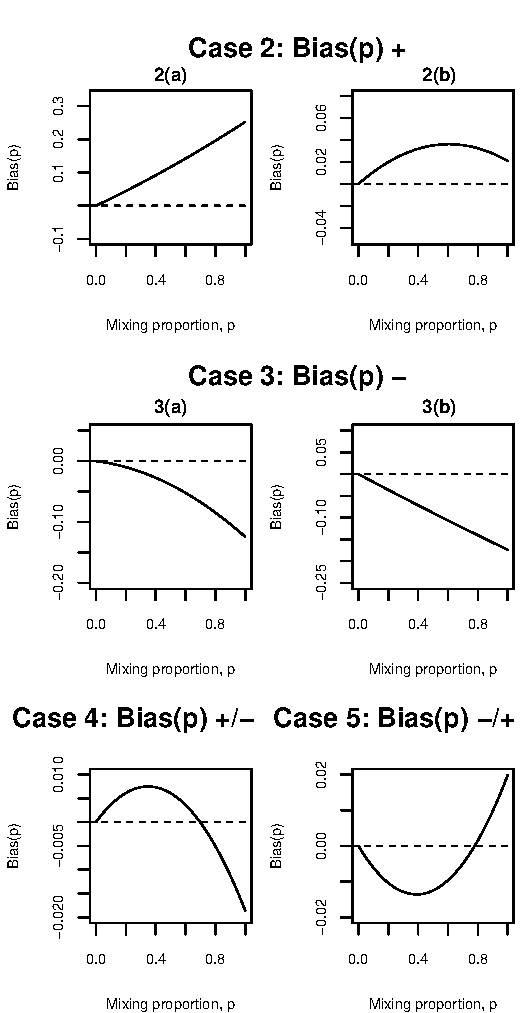
\includegraphics{images/tau_MO_graphs.pdf}
    %\caption{Possible scenarios for bias in Tau for a mixture of Marshall-Olkin distributions. These scenarios were produced using the parameter values in Table \ref{tab:tau}.}
    \caption{Using the values from Table \ref{tab:tau}, these are the possible scenarios for bias in Tau for a mixture of Marshall-Olkin distributions.}
    \label{fig:tauCases}
\end{figure}
\begin{figure}
    \centering
    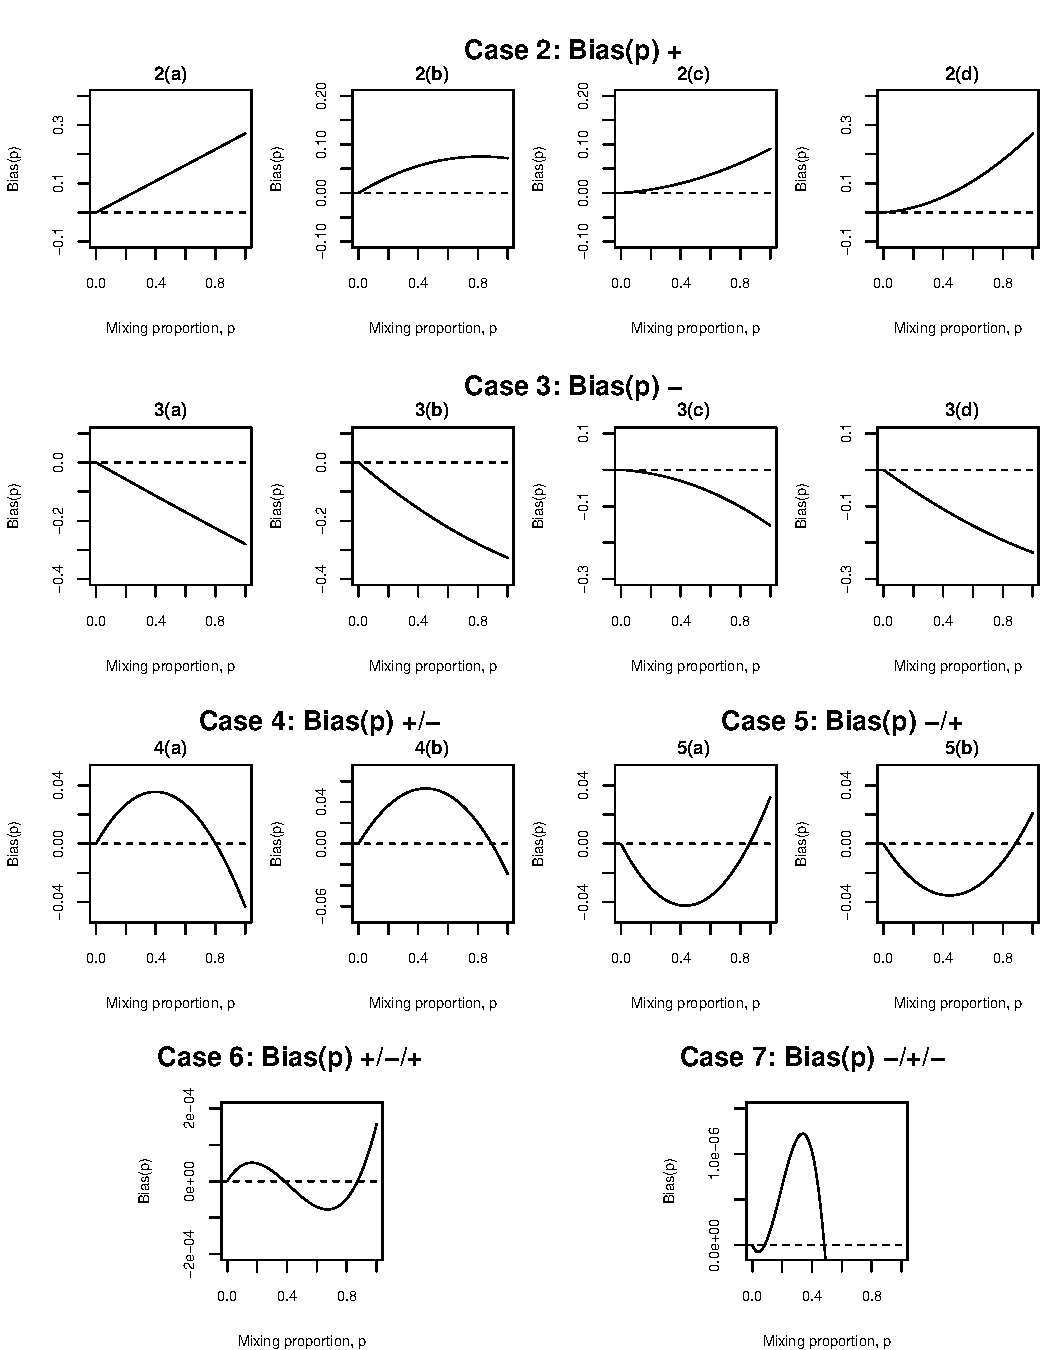
\includegraphics[scale=0.8]{images/rho_MO_graphs.pdf}
    %\caption{Possible scenarios for bias in Rho for a mixture of Marshall-Olkin distributions. These scenarios were produced using the parameter values in Table \ref{tab:rho}.}
    \caption{Using the values from Table \ref{tab:rho}, these are the possible scenarios for bias in Rho for a mixture of Marshall-Olkin distributions.}
    \label{fig:rhoCases}
\end{figure}
  \chapter{CONCLUSION}
\hspace{24pt} In conclusion, we have answered the result we set out to show. The bias for both rank correlation methods under mixture models are described as polynomials of degrees two and three. Using that result we elaborated and extended the potential by showing the different cases for both quadratics and cubic. The importance of this comes with application. If a researcher has potentially contaminated data, based on parameters they estimate, they may be able to predict whether the bias is positive or negative relative to the mixing proportion. That is, if their data follows a Marshall-Olkin distribution. However, after laying this foundation for bias analysis of rank correlation under mixtures, it could now be extended using different distributions or even multivariate distributions. A multivariate extension of Rho can be found in Trevor Camper's thesis {\it Essays on Mixture Models}, although his motivation is quite different \cite{camper2019}.

Along with our main results in Theorem \ref{theorem:main}, we also introduced a variety of different techniques throughout that readers may be unaware of. These include copulas, which are used extensively in the financial world, a generalized correlation coefficient, population extensions for Rho and Tau, Li's Theorem for CDFs, and some applications of Riemann-Stieljes integrals. The motivation of this project was to explore more techniques that statisticians can add to their toolbox when solving real-world problems. I believe this was accomplished in my thesis report. In reality, techniques are only as good as their ease to use and, with the R code that I provided and the analytical solution to the problems, it could make a successful statistical tool.
  \bibliography{bibliography.bib}

\end{document}